%\input{../../Plantillas/Libros/NotasDeClases}
\documentclass[mid,fleqn,draft,twoside]{notasdeclase}

\newcommand{\inte}[4]{\int_{#1}^{#2} #3\, d#4}
%\newcommand{\id}[1]{\mathfrak{#1}}
\newcommand{\an}[1]{\mathbb{#1}}
\newcommand{\ve}[1]{\bm{#1}}
\newcommand{\vcsp}[1]{\mathbb{#1}}
\newcommand{\V}{\mathbb{V}}
\newcommand{\F}{\mathbb{F}}
\newcommand{\Mn}[1]{\vcsp M_{n\t n}(\vcsp #1^n)}
\newcommand{\norm}{\lVert\phantom{a}\rVert}
\newcommand{\Norm}[1]{\left\lVert#1\right\rVert}
\newcommand{\iprod}{\langle\phantom{x},\phantom{x}\rangle}
\newcommand{\Iprod}[2]{\left\langle#1,#2\right\rangle}
\newcommand{\Bform}{(\phantom{a},\phantom{a})}
\newcommand{\bform}[2]{(#1,#2)}
\newcommand{\inv}{^{-1}}
\newcommand{\ort}{^\perp}
\renewcommand{\t}{\times}
\newcommand{\dt}[2]{#1_1 #2 #1_2 #2 \dots #2 #1_n}
\newcommand{\Dt}[2]{(#1_1+#2_1)^2 + \dots + (#1_n+#2_n)^2}
\newcommand{\pd}[1]{\frac{\partial}{\partial #1}}
\newcommand{\pdd}[2]{\dfrac{\partial #1}{\partial #2}}
\newcommand{\pds}[2]{\dfrac{\partial^2 #1}{\partial #2^2}} 
\newcommand{\pdx}[3]{\dfrac{\partial^2 #1}{\partial #2 \partial #3}}
\newcommand{\der}[1]{\frac{d}{d#1}}
\newcommand{\pol}[1]{#1_n x^n + #1_{n-1} x^{n-1} + \dots + #1_1 x + #1_0}
\newcommand{\Zn}{\mathbb{Z}/n\mathbb{Z}}
\newcommand{\Rn}{\mathbb{R}^n}
\newcommand{\Fn}{\mathbb{F}^n}
\newcommand{\Cn}{\mathbb{C}^n}
\newcommand{\Rm}{\mathbb{R}^m}
\newcommand{\R}{\mathbb{R}}
\newcommand{\Co}{\mathbb{C}}
\newcommand{\Z}{\mathbb{Z}}
\newcommand{\Q}{\mathbb{Q}}
\newcommand{\N}{\mathbb{N}}
\newcommand{\Ha}{\mathbb{H}}
\newcommand{\ihat}{\mathbb i}
\newcommand{\jhat}{\mathbb j}
\newcommand{\khat}{\mathbb k}

\begin{document}
\frontmatter
\begin{titlepage}
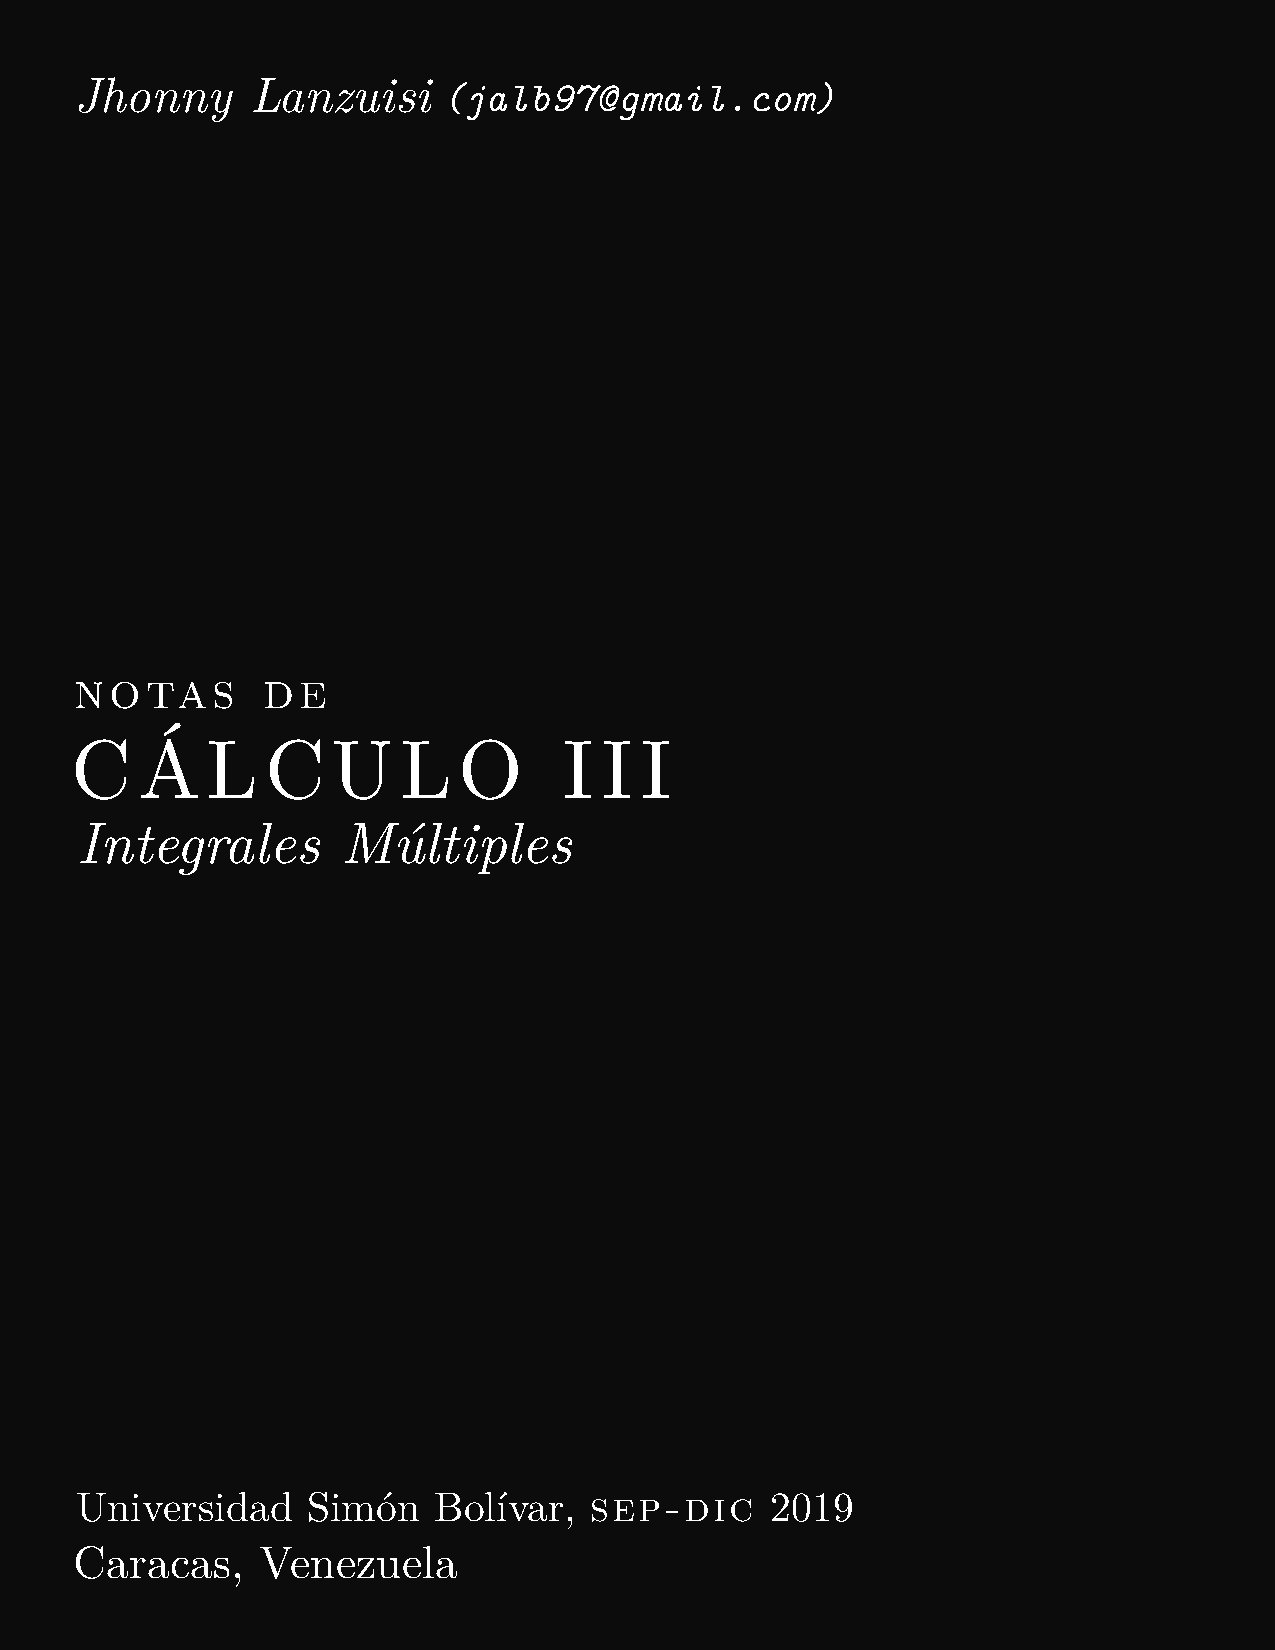
\includepdf[pages=-]{portada.pdf}
\end{titlepage}

%\begingroup
% a \clearpage will close the group and restore the meaning
%\let\clearpage\endgroup
\tableofcontents

\vspace{1em}
\begin{flushleft}
	\begin{tabular}[c]{rlr} 
%	\addlinespace[.5em]
	\multicolumn{3}{l}{\LARGE Evaluaciones} \\[1.5em]
	 { 1}er Parcial: & Semana 4 &({30}\%) \\
	 { 2}do Parcial: & Semana 8 &({35}\%) \\
	 { 3}er Parcial: & Semana 12 &({35}\%) \\
\end{tabular}

\end{flushleft}
%\twocolumn
\mainmatter
\setcounter{chapter}{-1}
\chapter{Preámbulos y Parametrizaciones}

\noindent
Este capítulo `cero' consiste de nociones básicas que son necesarias para los capítulos siguientes. 

\section{Integrales impropias}
%\clase{1}{lunes}{16/9}

\begin{defi}[convergencia]
	Sean $f$ y $g$ funciones reales y continuas en los intervalos $[a,\infty)$ y $[a,b]\setminus c$ respectivamente. Además, $ g(x) \to \pm\infty$ cuando $x\to c$. Entonces
	\begin{gather}
		\inte{a}{\infty}{f(x)}{x} = \lim\limits_{b\to\infty}\inte{a}{b}{f(x)}{x} \quad \text{y} \\
		\inte{a}{b}{g(x)}{x} = \lim\limits_{\beta\to c^{-}}\inte{a}{\beta}{g(x)}{x} + \lim\limits_{\alpha\to c^{+}}\inte{\alpha}{b}{g(x)}{x}.
	\end{gather}
	En caso de que los límites anteriores sean distintos de $\pm\infty$ diremos que las funciones convergen. En caso contrario diremos que divergen.
	
\end{defi}

\noindent
La condición, en la definición anterior, de que los limites no sean infinitos es de especial importancia en la ecuación (2). De no pedir esta condición obtendriamos expresiones sin sentido como $a=\infty-\infty$ para todo $a\in\R$.

El siguiente teorema, que tiene una contraparte directa cuando se trata de series infinitas, permitirá determinar si una integral converge o diverge sin la necesidad de calcular dicha integral. Esto es especialmente útil con funciones que no poseen antiderivadas, como $e^{x^2}$.

\begin{teo}[de comparación]
	Sean $f$ y $g$ dos funciones reales tales que $f(x)\leq g(x)$ para todo $x$ en el intervalo $[a,\infty)$ y, además, continuas en el intervalo abierto $(a,\infty)$. Entonces
	\begin{enumerate}
		\item Si $\inte{a}{\infty}{g(x)}{x}$ converge, entonces $\inte{a}{\infty}{f(x)}{x}$ también converge.
		\item Si $\inte{a}{\infty}{f(x)}{x}$ diverge, entonces $\inte{a}{\infty}{g(x)}{x}$ también diverge.
	\end{enumerate}
\end{teo}

Ahora, un ejemplo del teorema de comparación que involucra un función importante en probabilidades: la campana de Gau{\ss} (dada por $e^{-x^2}$).

\begin{ejem}
	Queremos determinar la convergencia de
	\[ \inte{0}{\infty}{e^{-x^2}}{x}. \]
	Compararemos con la función $e^{-x}$ de la cual conocemos bien su comportamiento. Primero notemos que, para todo $x\geq1$, $x^2\geq x$ implica $-x^2\leq -x$. De la última desigualdad se sigue claramente que $e^{-x^2}\leq e^{-x}$, y ya tenemos acotada la función problematica con una función que conocemos bien.
%		\marginpar{ 
%		\begin{minipage}{5.5cm}
%			\begin{figure}[H]
%				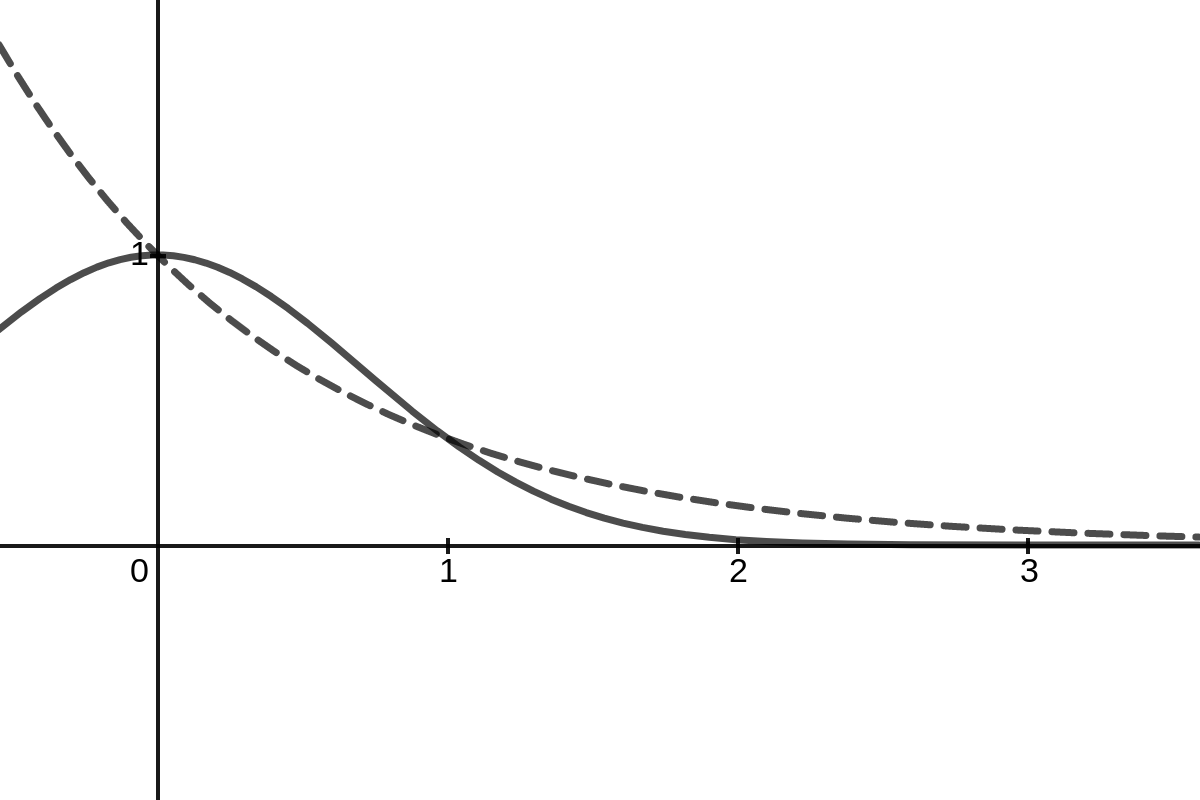
\includegraphics[width=.95\linewidth]{pics/g1}
%				\caption{Comparacion de $e^{-x^2}$ (linea continua) con $e^{-x}$ (segmentos de linea).}\label{ch0g1}
%			\end{figure}
%	\end{minipage}}
	Ahora, como la convergencia esta determinada por la `cola' de la forma $[a,\infty)$, podemos considerar la convengencia de $e^{-x^2}$ tomando el intervalo $[1,\infty)$. Queda entonces por determinar la convergencia de $e^{-x}$ y luego, por el teorema de comparación, tendremos que $e^{-x^2}$ converge.
	
	La convergencia de $e^{-x}$ es sencilla:
	\begin{align*}
		\inte{1}{\infty}{e^{-x}}{x} &= \lim\limits_{b\to\infty}\inte{1}{b}{e^{-x}}{x} \\ 
		&=  \lim\limits_{b\to\infty}  e^{-x} \bigg|^b_1 \\
		&= e\inv - \lim\limits_{b\to\infty} e^{-b}  \\
		&= e\inv.
	\end{align*}

	El argumento anterior puede verse gráficamente en la figura~\ref{ch0g1}.\\

\begin{center}
			\begin{figure}[H]\centering
			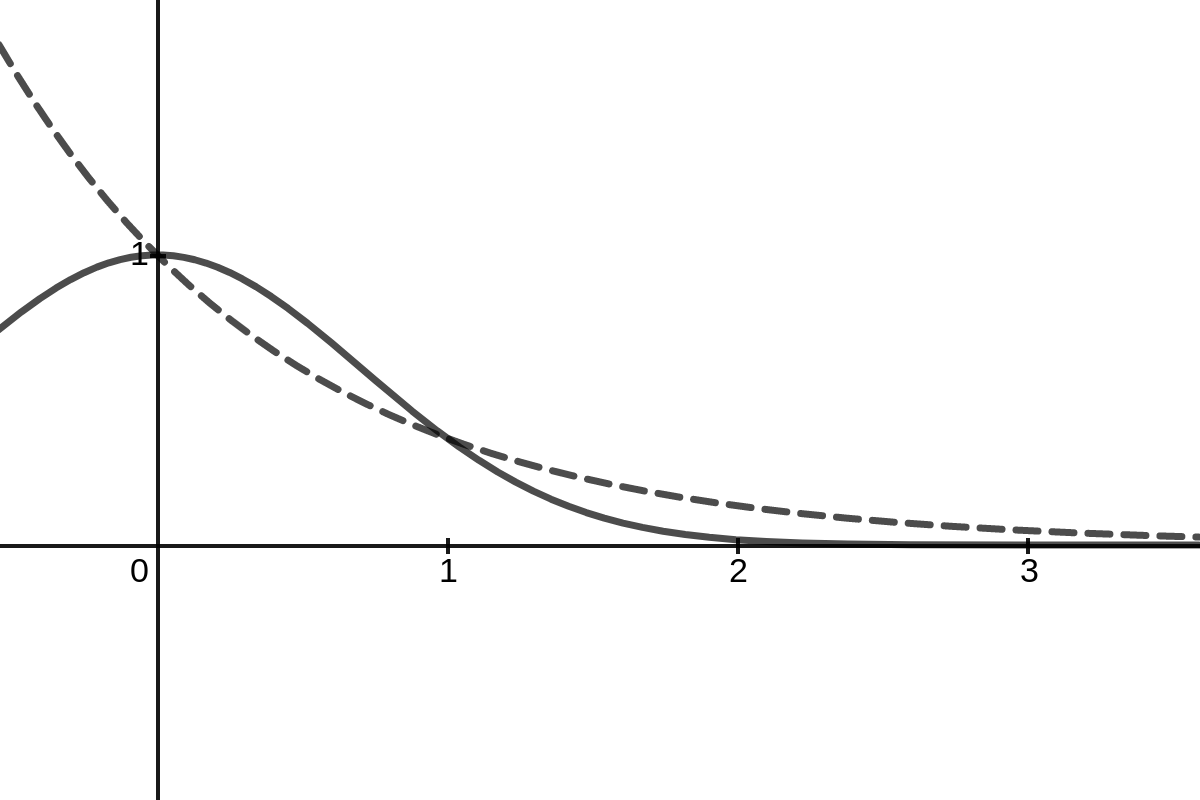
\includegraphics[width=.6\linewidth]{pics/g1}
			\caption{Comparacion de $e^{-x^2}$ (linea continua) con $e^{-x}$ (segmentos de linea).}\label{ch0g1}
		\end{figure}
\end{center}

\end{ejem}
\section{Integración respecto a un parámetro}
%\clase{2}{jueves}{19/9}
\noindent
La continuidad uniforme será fundamental para la \emph{integración respecto a un parámetro}, que es una herramienta útil en el cálculo de integrales complicadas o irresolubles. 

\begin{defi}[continuidad uniforme]\label{cont-uniforme}
	Si la función $f\colon I\subset\R\to\R$ es continua, decimos que es \textup{\textsf{\textsc{uniformemente continua}}} en un $x_0\in I$, si existe un $\epsilon>0$ tal que para todo $\delta$ se cumple que
	\[ |x-x_0| <\delta\quad\text{implica}\quad |f(x)-f(x_0)| <\epsilon, \]
	es decir, que $\epsilon$ no depende de $x$.
\end{defi}

\begin{ejem}\label{ejeme-x}
%		\marginpar{
%		\begin{minipage}{5.5cm}
%			\begin{figure}[H]\centering
%				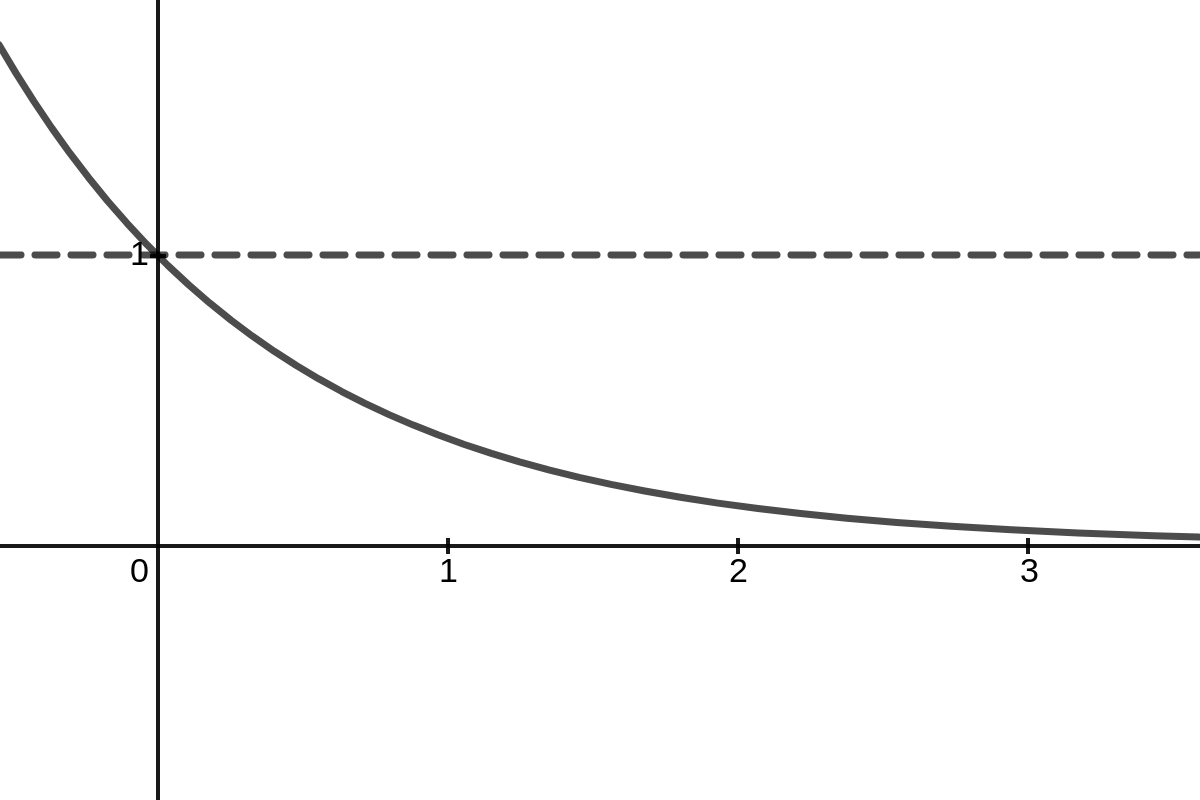
\includegraphics[width=.95\linewidth]{pics/g2}\\ 
%				\caption{Gráfico de $e^{-x}$ (linea continua) con su asíntota horizontal.}\label{ch0g2}
%			\end{figure}
%	\end{minipage}}
	Queremos ver si la función $f(x) = e^{-x}$ es uniformente continua en el intervalo $[0,\infty)$.
	
	Por el teorema del valor medio\footnote{explicar teorema} tenemos
	\[ |e^x-e^{-x_0}| = |e^{-x_1} (x-x_0)|  = e^{-x_1}| (x-x_0)|. \]
	Como $x_1\in [x_0,x]\subset[0,\infty)$ y $e^{-x}$ es estrictamente decreciente en $[0,\infty)$, se sigue que $e^{-x_1} \leq e^0=1$ y sustituyendo esto en la ecuación anterior
	\[ |e^x - e^{x_0}|\leq 1|x-x_0| <\delta. \]
	Por lo tanto basta con tomar $\epsilon=1$ para tener la continuidad uniforme.
	
	Lo que ocurre gráficamente es que $e^{-x}$ esta acotada superior e inferiormente como lo muestra la figura~\ref{ch0g2}
\end{ejem}

\begin{minipage}{.48\linewidth}
	\begin{figure}[H]\centering
		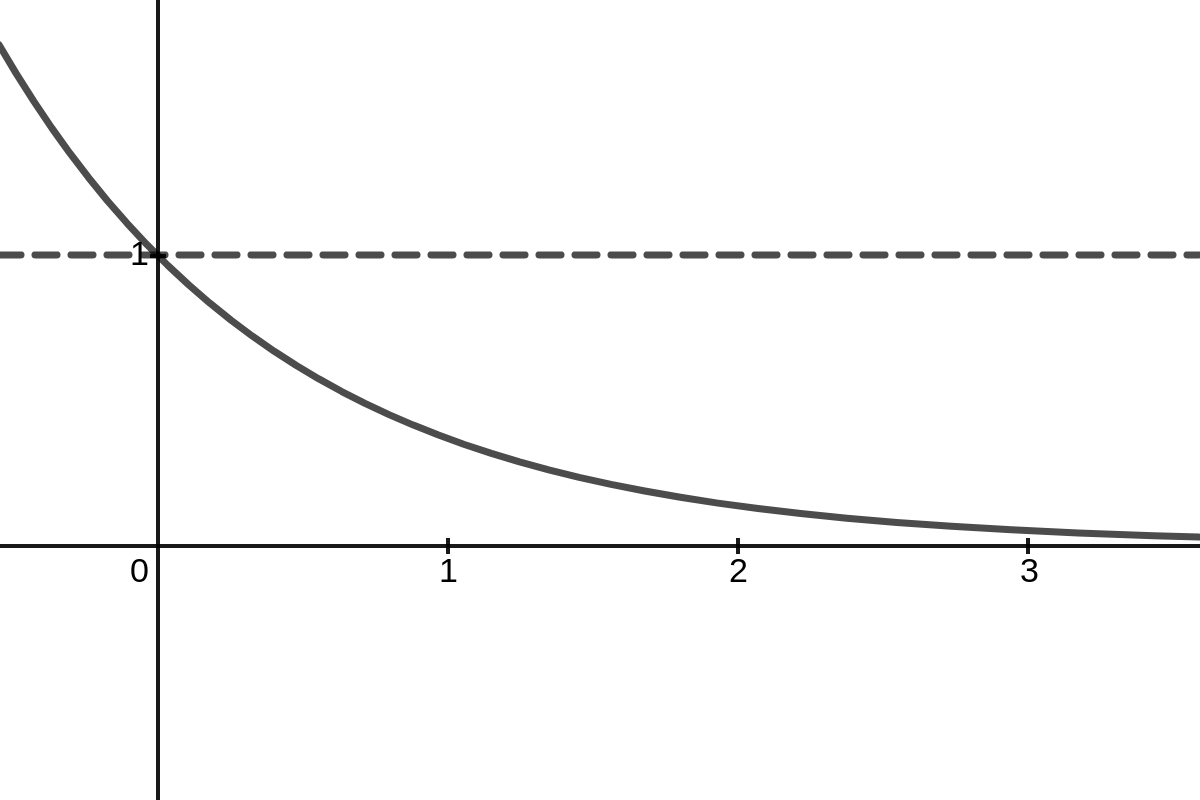
\includegraphics[width=.95\linewidth]{pics/g2}\\ 
		\caption{Gráfico de $e^{-x}$ (linea continua) con su asíntota horizontal.}\label{ch0g2}
	\end{figure}
\end{minipage}
\begin{minipage}{.48\linewidth}
	\begin{figure}[H]\centering
		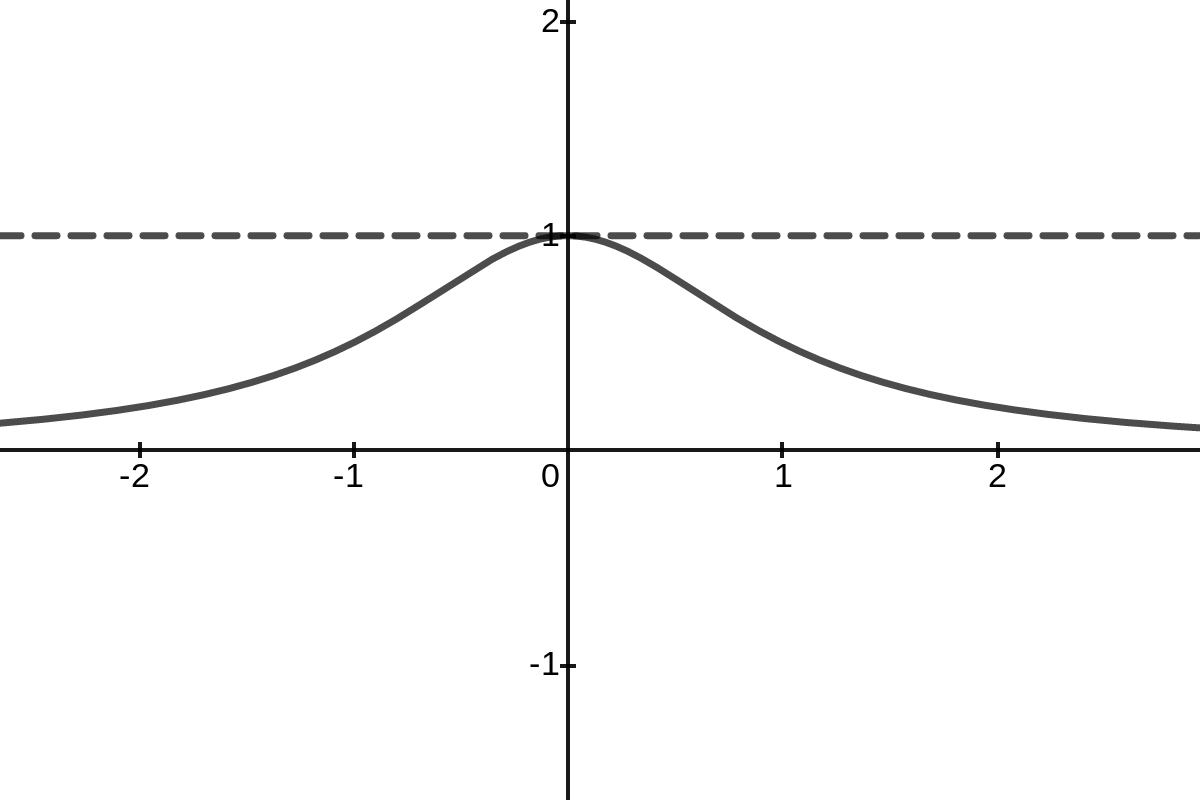
\includegraphics[width=.95\linewidth]{pics/g3}\\ 
		\caption{Gráfico de $\dfrac{1}{1+x^2}$ (linea continua) con su asíntota horizontal.}
	\end{figure}
\end{minipage}
\begin{cejem}
	Sea $f(x) = 1/x$ definida en el intervalo $(0,1)$. Esta función $f$ es continua, sin embargo, no es uniformemente continua. Veamos que
	\[ \left| \frac 1x - \frac{1}{x_0} \right| = \left| \frac{x-x_0}{xx_0} \right|. \]
	Si $|x|<1/2$ entonces $1/x>2$, y esto ocurre también para $x_0$: $1/x_0>2$, de donde
	\[ \left| \frac 1x - \frac{1}{x_0} \right| = \frac{1}{xx_0}|x-x_0| > 4 |x-x_0|\geq\epsilon \]
	por lo que no existe un único $\epsilon$ que cumpla con la definición~\ref{cont-uniforme}.
\end{cejem}
\begin{ejem}
	Consideremos la función
	\[ f(x)=\frac{1}{1+x^2}. \]
	Teniendo en cuenta el gráfico de la función, es decir, que esta acotada; ocurrirá lo mismo que en el ejemplo~\ref{ejeme-x}.
%		\marginpar{
%		\begin{minipage}{5.5cm}
%		\begin{figure}[H]\centering
%	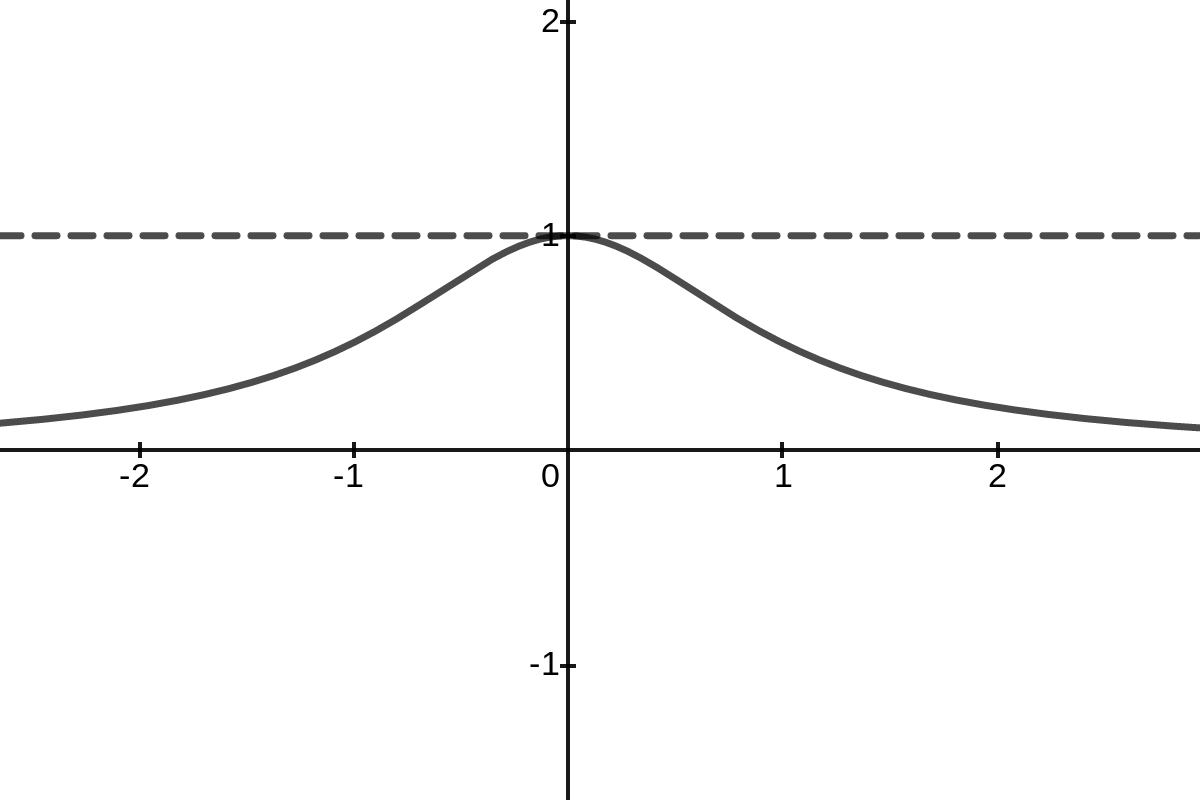
\includegraphics[width=.95\linewidth]{pics/g3}\\ 
%	\caption{Gráfico de $\dfrac{1}{1+x^2}$ (linea continua) con su asíntota horizontal.}
%\end{figure}
%	\end{minipage}}
\end{ejem}

A continuación está el teorema central de esta clase:
\begin{teo}[integración respecto a un parámetro]
	Sea $f$ una función, que va del subconjunto $I_x\t I_a$ de $\R^2$ a $\R$, definida como $f(x) = (x,a)$ para $x\in I_x$ y un $a$ \emph{fijo} en $I_a$. Si $f$ es uniformemente continua en $I_x$, entonces
	\begin{gather}
	\der{a} \inte{u}{v}{f(x,a)}{x} = \inte{u}{v}{\pd{a} f(x,a)}{x} \quad\text{y} \\ 
	\der{a} \inte{u(a)}{v(a)}{f(x,a)}{x} = \inte{u(a)}{v(a)}{\pd{a} f(x,a)}{x}  \\
	\hspace{9em} + f(v(a),a)v'(a) - f(u(a),a)u'(a). \nonumber
	\end{gather}
\end{teo}

El siguiente es un ejemplo, un tanto complicado, de como usar la técnica del teorema anterior.
\begin{ejem}
	Calcular, usando integración respecto a un parámetro,
	\[ \inte{0}{\infty}{\frac{\arctan(ax)}{x(1+x^2)}}{x}. \]
	Hagamos
	\[ g(a)= \inte{0}{\infty}{\frac{\arctan(ax)}{x(1+x^2)}}{x} = \inte{0}{\infty}{f(x,a)}{x} \]
	donde $f(x,a)$ cumple con:
	\begin{itemize}
		\item $\displaystyle\lim\limits_{x\to 0} \frac{\arctan(ax)}{x} = \lim\limits_{x\to0}\frac{1}{1+(ax)^2} = \frac{a}{1+0} = a$
		\item $\displaystyle\left| \frac{1}{1+x^2} \right| = \frac{1}{1+x^2}\leq\frac{1}{1+0}=1$
	\end{itemize}
	por lo que $f(x,a)$ es el producto de una función acotada por una función uniformemente continua, lo que implica que $f(x,a)$ es uniformemente continua. Se cumplen entonces las hipótesis del teorema y podemos aplicarlo:
	\begin{align*}
		g'(a) &= \der{a}\inte{0}{\infty}{\frac{\arctan(ax)}{x(1+x^2)}}{x} \\
		      &= \inte{0}{\infty}{\pd{a}\frac{\arctan(ax)}{x(1+x^2)}}{x} \\
		      &= \inte{0}{\infty}{\frac{\cancel{x}}{\cancel{x}(1+x^2)(1+a^2x^2)}}{x} \\
		      &= \inte{0}{\infty}{\frac{1}{(1+x^2)(1+a^2x^2)}}{x}.
	\end{align*}
	Pero:
	\begin{align*}
		\frac{1}{\cancel{(1+x^2)(1+a^2x^2)}} &= \frac{B}{1+x^2} + \frac{D}{1+a^2x^2} \\
											 &= \frac{B(1+a^2x^2) + D(1+x^2)}{\cancel{(1+x^2)(1+a^2x^2)}} .
	\end{align*}
	De donde se sigue que $1=(B+D) + (a^2B+D)x^2$ y se obtiene el siguiente sistema de ecuaciones:
	\[ 
	\begin{cases}
	B+D  =1 \\
	a^2B+D=0,
	\end{cases}
	 \]
	 cuyas soluciones son
	 \[ B=\frac{1}{1-a^2}\quad\text{y}\quad D=\frac{-a^2}{1+a^2x^2}. \]
	 Volviendo a $g'(a)$, tenemos
	 
	 \begin{align*}
	 	g'(a) &= \frac{1}{1-a^2}\int_{0}^{\infty}\frac{\mathrm dx}{1+x^2} - \frac{a}{1-a^2}\int_{0}^{\infty}\frac{a\,\mathrm dx}{1+a^2x^2} \\
	 	      &= \frac{1}{1-a^2}\lim\limits_{b\to\infty}\arctan(x)\bigg|_0^b \\
	 	      &\phantom{=}\hspace{6.5em}- \frac{a}{1-a^2}\lim\limits_{b\to\infty}\arctan(ax)\bigg|_0^b \\
	 	      &=\frac{\pi}{2}\frac{1}{1-x^2} - \frac{\pi}{2}\frac{a}{1-a^2} \\
	 	      &=\frac{\pi}{2}\frac{1}{1+a}.
	 \end{align*}
	 
	 Esto implica que
	 \begin{align*}
	 	g(a) &= \inte{0}{\infty}{\frac{\pi}{2}\frac{1}{1+t}}{t} \\
	 		 &= \frac{\pi}{2}\log(1+t)\bigg|_{t=0}^{t=a} \\
	 		 &= \frac{\pi}{2}\log(1+a).
	 \end{align*}
\end{ejem}
%\clase{3}{viernes}{20/9}
En el siguiente ejemplo se calcula la integral de la campana de Gau{\ss}.
\begin{ejem}
	Sean
	\[ f(x)=\bigg(\inte{0}{x}{-e^{-t^2}}{t}\bigg)^2\quad\text{y}\quad g(x)=\inte{0}{1}{\frac{e^{-x^2(1+t^2)}}{1+t^2}}{t}. \]
	\begin{enumerate}
		\item Demostrar que $f(x)+g(x)=\text{ctte}$.
		\item Usa la parte anterior para calcular $\inte{0}{\infty}{e^{-t^2}}{t}.$
	\end{enumerate}
	Veamos cada parte.
	\begin{enumerate}
		\item Empecemos calculando la derivada de $f$:
		\begin{align*}
			\frac{\mathrm df}{\mathrm dx} &=\bigg(2\inte{0}{x}{-e^{-t^2}}{t}\bigg)\bigg(\der{t}\inte{0}{x}{-e^{-t^2}}{t}\bigg) \\
			&= 2\inte{0}{x}{e^{-t^2}e^{-x^2}}{t} \\
			&=2\inte{0}{x}{e^{-(t^2+x^2)}}{t}.
		\end{align*}
		Ahora, para calcular la derivada de $g$, debemos ver primero que es uniformemente continua. Hagamos
		\[ g(x)=\inte{0}{1}{\phi_x(t)}{t}. \] 
		Como el intervalo $I_t=[0,1]$ es cerrado y acotado y $\phi_x(t)$ es continua en la variable $t$, por el teorema de Bolzano $\phi_x(t)$ alcanza máximos y mínimos y entonces es uniformemente continua. Podemos usar derivación paramétrica:
		\begin{align*}
			\frac{\mathrm dg}{\mathrm dx} &= \inte{0}{1}{\pd{x}\frac{e^{-x^2(1+t^2)}}{1+t^2}}{t} \\
										  &= \inte{0}{1}{-2x\cancel{(1+t^2)}\frac{e^{-x^2(1+t^2)}}{\cancel{1+t^2}}}{t} \\
										  &= -2\inte{0}{1}{e^{-x^2+(xt)^2}}{t}.
		\end{align*}
		Necesitamos que $f'$ y $g'$ se parezcan más para poder hacer su suma cero. Comencemos haciendo
		\[ \frac{\mathrm df}{\mathrm dx} = 2\inte{0}{x}{e^{-(u^2+t^2)}}{u}, \]
		y luego el cambio $u=xt$ en $g'$ para obtener
		\[ \frac{\mathrm dg}{\mathrm dx} = -2\inte{0}{x}{e^{-(u^2+t^2)}}{u} = -\frac{\mathrm df}{\mathrm dx}\]
		 y queda demostrado que $f+g$ es constante. Para determinar la constante hagamos 
		\[ h(x)  = f(x)+g(x) \]
		y luego $h(x)=h(x_0)$ para cualquier $x_0\in\R$ elegido convenientemente. Elijamos $x_0=0$, entonces
		\begin{align*}
			\mathrm{ctte} &= h(0)\\
						  &= \bigg(\inte{0}{0}{-e^{-t^2}}{t}\bigg)^2 + \inte{0}{1}{\frac{e^{-0^2(1+t^2)}}{1+t^2}}{t} \\
						  &= \inte{0}{1}{\frac{1}{1+t^2}}{t} \\
						  &= \arctan(1)-\arctan(0) \\
						  &=\frac \pi 4.
		\end{align*}
		\item Se puede demostrar que 
		\[ \lim\limits_{x\to\infty}\inte{a}{b}{\phi_x(t)}{t} =\inte{a}{b}{ \lim\limits_{x\to\infty}\phi_x(t)}{t}. \]
		Pero
		\[ \lim\limits_{x\to\infty}\frac{e^{-x^2(1+t^2)}}{1+t^2} = \frac{0}{1+t^2} = 0. \]
		Tomando límites en la respuesta de la parte anterior
		
		\[ \lim\limits_{x\to\infty}\bigg(\inte{0}{x}{-e^{-t^2}}{t}\bigg)^2 + \lim\limits_{x\to\infty}\inte{0}{1}{\frac{e^{-x^2(1+t^2)}}{1+t^2}}{t} = \frac{\pi}{4} \]
		
		de donde se sigue que
		\[ \bigg(\inte{0}{\infty}{-e^{-t^2}}{t}\bigg)^2 + 0 = \frac{\pi}{4} \]
		y finalmente, tomando raíces cuadradas,
		\[ \inte{0}{\infty}{-e^{-t^2}}{t} = \frac{\sqrt{\pi}}{2}. \]
	\end{enumerate}
\end{ejem}

\section{Parametrizaciones clásicas}

\begin{defi}[parametrización]
	Sean $\Omega$ y $\Lambda$ dos objetos geométricos, con $\Omega\subset\Rn$ y $\Lambda\subset\Rm$ ($1\leq n,m\leq3$) (En general $\Lambda$ y $\Omega$ pueden ser: puntos, líneas, superficies planas o curvilíneas, volúmenes sólidos). Una parametrización es una aplicación $\Phi\colon\Omega\to\Lambda$ cuya acción no conviene estudiar a partir de $\ve v= \Phi(\ve u)$ y su gráfico $\mathcal{G}_\Phi$, sino que conviene estudiarla por el mapeo de la figura~\ref{ch0d1}.
%	
\tikzset{every picture/.style={line width=0.75pt}} %set default line width to 0.75pt        
\marginnote{
	\begin{minipage}{5.5cm}
		\begin{figure}[H]\centering
			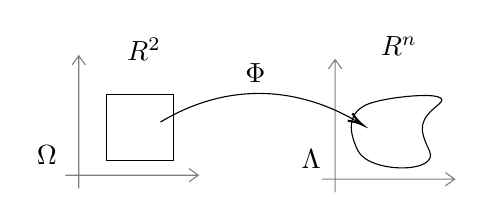
\begin{tikzpicture}[x=0.6pt,y=0.6pt,yscale=-1,xscale=1,scale=.80]
			%uncomment if require: \path (0,237); %set diagram left start at 0, and has height of 237
			
			%Shape: Axis 2D [id:dp3785820715688062] 
			\draw [color={rgb, 255:red, 128; green, 128; blue, 128 }  ,draw opacity=1 ] (50,168) -- (150,168)(60,78) -- (60,178) (143,163) -- (150,168) -- (143,173) (55,85) -- (60,78) -- (65,85)  ;
			%Shape: Axis 2D [id:dp47611229523996135] 
			\draw [color={rgb, 255:red, 128; green, 128; blue, 128 }  ,draw opacity=1 ] (243,171) -- (343,171)(253,81) -- (253,181) (336,166) -- (343,171) -- (336,176) (248,88) -- (253,81) -- (258,88)  ;
			%Shape: Square [id:dp6078316056685962] 
			\draw   (81,107) -- (131,107) -- (131,157) -- (81,157) -- cycle ;
			%Curve Lines [id:da3192192248631224] 
			\draw    (121.5,128) .. controls (172.49,97.31) and (225.92,100.92) .. (272.1,129.14) ;
			\draw [shift={(273.5,130)}, rotate = 211.95] [color={rgb, 255:red, 0; green, 0; blue, 0 }  ][line width=0.75]    (10.93,-3.29) .. controls (6.95,-1.4) and (3.31,-0.3) .. (0,0) .. controls (3.31,0.3) and (6.95,1.4) .. (10.93,3.29)   ;
			
			%Shape: Regular Polygon [id:dp6479810872135613] 
			\draw   (277.12,114.69) .. controls (290.25,108.9) and (345.22,103.1) .. (330.93,114.69) .. controls (316.63,126.28) and (315.46,132.08) .. (323.91,149.46) .. controls (332.36,166.85) and (278.55,166.85) .. (270.1,149.46) .. controls (261.65,132.08) and (263.99,120.49) .. (277.12,114.69) -- cycle ;
			
			% Text Node
			\draw (109,73) node   {$\R^2$};
			% Text Node
			\draw (301,71) node   {$\R^n$};
			% Text Node
			\draw (36,153) node   {$\Omega $};
			% Text Node
			\draw (235,156) node   {$\Lambda $};
			% Text Node
			\draw (193,91) node   {$\Phi $};
			
			
			\end{tikzpicture}
			\caption{Mapeo de una parametrización.}\label{ch0d1}
		\end{figure}
\end{minipage}}

El cual se define como

\[
	\ve v = \begin{pmatrix}
	v_1 \\ v_2 \\ \vdots \\ v_m
	\end{pmatrix} = 
	\Phi\begin{pmatrix}
	u_1\\u_2\\ \vdots\\ u_n
	\end{pmatrix} 
	\iff \begin{cases}
	v_1 = \phi_1(\dt{u}{,}) \\
	v_2 = \phi_2(\dt{u}{,}) \\
	\vdots \\
	v_m = \phi_m(\dt{u}{,}).
	\end{cases}
\]

\end{defi}

Nos interesan principalmente cinco casos concretos:


\paragraph{caso 1-2 curvas planas} Tomemos $\Phi\colon\Omega\subset\R_t\to\R^2_{xy}$. Entonces las coordenadas $x,y$ de un vector se escriben con respecto a $\Phi$ y a $\Phi'$, de la siguiente manera
%	\marginnote{
	\begin{minipage}{5.5cm}
		\begin{figure}[H]\centering
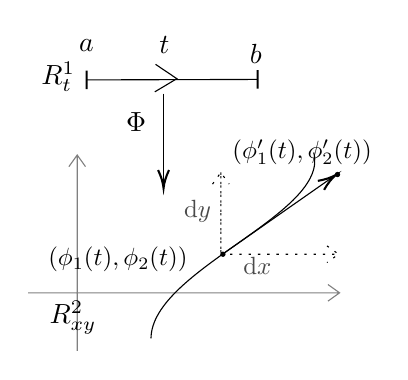
\begin{tikzpicture}[x=0.6pt,y=0.6pt,yscale=-1,xscale=1]
%Shape: Axis 2D [id:dp41021135976261514] 
\draw [color={rgb, 255:red, 128; green, 128; blue, 128 }  ,draw opacity=1 ] (5,256) -- (192.5,256)(34.5,173) -- (34.5,291) (185.5,251) -- (192.5,256) -- (185.5,261) (29.5,180) -- (34.5,173) -- (39.5,180)  ;
%Straight Lines [id:da5315594181633504] 
\draw    (143.15,127.48) -- (40.14,127.77) ;
\draw [shift={(40.14,127.77)}, rotate = 359.83000000000004] [color={rgb, 255:red, 0; green, 0; blue, 0 }  ][line width=0.75]    (0,5.59) -- (0,-5.59)   ;
\draw [shift={(143.15,127.48)}, rotate = 359.83000000000004] [color={rgb, 255:red, 0; green, 0; blue, 0 }  ][line width=0.75]    (0,5.59) -- (0,-5.59)   ;
\draw   (81.67,118.39) -- (94.51,127.04) -- (81.22,134.97) ;

%Shape: Circle [id:dp36661837654320517] 
\draw  [fill={rgb, 255:red, 0; green, 0; blue, 0 }  ,fill opacity=1 ] (123.5,232.75) .. controls (123.5,232.06) and (122.94,231.5) .. (122.25,231.5) .. controls (121.56,231.5) and (121,232.06) .. (121,232.75) .. controls (121,233.44) and (121.56,234) .. (122.25,234) .. controls (122.94,234) and (123.5,233.44) .. (123.5,232.75) -- cycle ;
%Shape: Circle [id:dp3341593596220296] 
\draw  [fill={rgb, 255:red, 0; green, 0; blue, 0 }  ,fill opacity=1 ] (192.5,184.75) .. controls (192.5,184.06) and (191.94,183.5) .. (191.25,183.5) .. controls (190.56,183.5) and (190,184.06) .. (190,184.75) .. controls (190,185.44) and (190.56,186) .. (191.25,186) .. controls (191.94,186) and (192.5,185.44) .. (192.5,184.75) -- cycle ;
%Shape: Axis 2D [id:dp8708604035951039] 
\draw [dash pattern={on 0.84pt off 2.51pt}] (121,232.75) -- (191.93,232.75)(121,183.53) -- (121,232.75) -- cycle (184.93,227.75) -- (191.93,232.75) -- (184.93,237.75) (116,190.53) -- (121,183.53) -- (126,190.53)  ;
%Straight Lines [id:da5074920899678971] 
\draw    (122,232.75) -- (188.61,186.15) ;
\draw [shift={(190.25,185)}, rotate = 505.02] [color={rgb, 255:red, 0; green, 0; blue, 0 }  ][line width=0.75]    (10.93,-3.29) .. controls (6.95,-1.4) and (3.31,-0.3) .. (0,0) .. controls (3.31,0.3) and (6.95,1.4) .. (10.93,3.29)   ;

%Curve Lines [id:da6202345516128739] 
\draw    (78.93,283.43) .. controls (79.37,241.87) and (186.93,208.53) .. (176.93,171.53) ;


%Straight Lines [id:da48049376839429636] 
\draw    (86.5,136) -- (86.5,191) ;
\draw [shift={(86.5,193)}, rotate = 270] [color={rgb, 255:red, 0; green, 0; blue, 0 }  ][line width=0.75]    (10.93,-3.29) .. controls (6.95,-1.4) and (3.31,-0.3) .. (0,0) .. controls (3.31,0.3) and (6.95,1.4) .. (10.93,3.29)   ;


% Text Node
\draw (40,107) node   {$a$};
% Text Node
\draw (142,112) node   {$b$};
% Text Node
\draw (87,107) node   {$t$};
% Text Node
\draw (70,153) node   {$\Phi $};
% Text Node
\draw (59,236) node [scale=0.9]  {$( \phi _{1}( t) ,\phi _{2}( t))$};
% Text Node
\draw (169.93,171.53) node [scale=0.9]  {$( \phi '_{1}( t) ,\phi '_{2}( t))$};
% Text Node
\draw (143,240) node [scale=0.9,color={rgb, 255:red, 74; green, 74; blue, 74 }  ,opacity=1 ]  {$\mathrm{d} x$};
% Text Node
\draw (107,207) node [scale=0.9,color={rgb, 255:red, 74; green, 74; blue, 74 }  ,opacity=1 ]  {$\mathrm{d} y$};
% Text Node
\draw (23,126) node   {$\R^{1}_{t}$};
% Text Node
\draw (32,271) node   {$\R^{2}_{xy}$};
\end{tikzpicture}
			\caption{Mapeo del caso 1-2.}\label{ch0d2}
		\end{figure}
\end{minipage}}[-4em]
\[ 
\begin{cases}
x = \phi_1(t) \\
y = \phi_2(t) \\
\end{cases} \quad\text{y}
\quad\begin{cases}\displaystyle
\frac{\mathrm dx}{\mathrm dt} = \phi_1'(t) \\[.8em] \displaystyle
\frac{\mathrm dy}{\mathrm dt} = \phi_2'(t)
\end{cases}
 \]
y el mapeo correspondiente esta dado en la figura~\ref{ch0d2}.

  \paragraph{caso 1-3 curvas en el espacio} Tomemos $\Phi\colon\Omega\subset\R^1_t\to\R^3_{xyz}$. Entonces las coordenadas $x,y,z$ de un vector se escriben con respecto a $\Phi$ y a $\Phi'$ de la siguiente manera
%  \marginnote{
	\begin{minipage}{5.5cm}
		\begin{figure}[H]\centering
	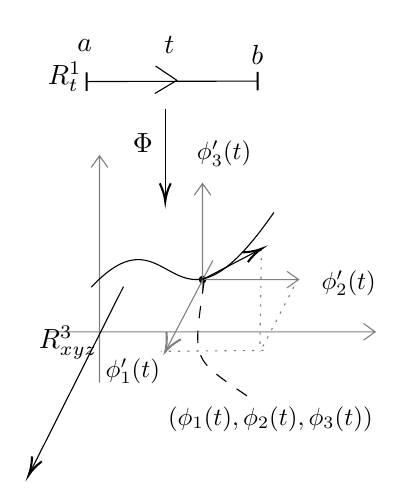
\begin{tikzpicture}[x=0.6pt,y=0.6pt,yscale=-1,xscale=1]
	%uncomment if require: \path (0,439); %set diagram left start at 0, and has height of 439
	
	%Straight Lines [id:da010258542781164337] 
	\draw    (142.15,171.48) -- (39.14,171.77) ;
	\draw [shift={(39.14,171.77)}, rotate = 359.83000000000004] [color={rgb, 255:red, 0; green, 0; blue, 0 }  ][line width=0.75]    (0,5.59) -- (0,-5.59)   ;
	\draw [shift={(142.15,171.48)}, rotate = 359.83000000000004] [color={rgb, 255:red, 0; green, 0; blue, 0 }  ][line width=0.75]    (0,5.59) -- (0,-5.59)   ;
	\draw   (80.67,162.39) -- (93.51,171.04) -- (80.22,178.97) ;
	
	%Shape: Axis 2D [id:dp6889745385829058] 
	\draw [color={rgb, 255:red, 128; green, 128; blue, 128 }  ,draw opacity=1 ] (16,322.5) -- (212.93,322.5)(46.93,216.5) -- (46.93,353.04) (205.93,317.5) -- (212.93,322.5) -- (205.93,327.5) (41.93,223.5) -- (46.93,216.5) -- (51.93,223.5)  ;
	%Shape: Boxed Line [id:dp16438192577140776] 
	\draw    (61.33,295.28) -- (5.18,407.02) ;
	\draw [shift={(4.28,408.8)}, rotate = 296.68] [color={rgb, 255:red, 0; green, 0; blue, 0 }  ][line width=0.75]    (10.93,-3.29) .. controls (6.95,-1.4) and (3.31,-0.3) .. (0,0) .. controls (3.31,0.3) and (6.95,1.4) .. (10.93,3.29)   ;
	
	%Shape: Circle [id:dp7087171813046038] 
	\draw  [fill={rgb, 255:red, 0; green, 0; blue, 0 }  ,fill opacity=1 ] (110.93,291.03) .. controls (110.93,289.95) and (110.05,289.07) .. (108.97,289.07) .. controls (107.88,289.07) and (107,289.95) .. (107,291.03) .. controls (107,292.12) and (107.88,293) .. (108.97,293) .. controls (110.05,293) and (110.93,292.12) .. (110.93,291.03) -- cycle ;
	%Shape: Axis 2D [id:dp3359608795022041] 
	\draw [color={rgb, 255:red, 128; green, 128; blue, 128 }  ,draw opacity=1 ] (102.54,291.03) -- (166.79,291.03)(108.97,233.21) -- (108.97,297.46) (159.79,286.03) -- (166.79,291.03) -- (159.79,296.03) (103.97,240.21) -- (108.97,233.21) -- (113.97,240.21)  ;
	%Straight Lines [id:da9864853885071442] 
	\draw [color={rgb, 255:red, 128; green, 128; blue, 128 }  ,draw opacity=1 ]   (115.15,279.5) -- (87.41,332.66) ;
	\draw [shift={(86.48,334.43)}, rotate = 297.56] [color={rgb, 255:red, 128; green, 128; blue, 128 }  ,draw opacity=1 ][line width=0.75]    (10.93,-4.9) .. controls (6.95,-2.3) and (3.31,-0.67) .. (0,0) .. controls (3.31,0.67) and (6.95,2.3) .. (10.93,4.9)   ;
	
	%Shape: Boxed Line [id:dp9016333005766098] 
	\draw [color={rgb, 255:red, 128; green, 128; blue, 128 }  ,draw opacity=1 ] [dash pattern={on 0.84pt off 2.51pt}]  (166.59,290.5) -- (143.48,334.77) ;
	
	
	%Shape: Boxed Line [id:dp3804166141611265] 
	\draw [color={rgb, 255:red, 128; green, 128; blue, 128 }  ,draw opacity=1 ] [dash pattern={on 0.84pt off 2.51pt}]  (145.8,333.67) -- (83.84,334.26) ;
	
	
	%Straight Lines [id:da6259198083466047] 
	\draw [color={rgb, 255:red, 128; green, 128; blue, 128 }  ,draw opacity=1 ] [dash pattern={on 0.84pt off 2.51pt}]  (144.44,272.48) -- (143.48,334.43) ;
	
	
	%Straight Lines [id:da43876051555056905] 
	\draw    (108.97,291.03) -- (142.66,273.4) ;
	\draw [shift={(144.44,272.48)}, rotate = 512.38] [color={rgb, 255:red, 0; green, 0; blue, 0 }  ][line width=0.75]    (10.93,-3.29) .. controls (6.95,-1.4) and (3.31,-0.3) .. (0,0) .. controls (3.31,0.3) and (6.95,1.4) .. (10.93,3.29)   ;
	
	%Curve Lines [id:da9461526898510314] 
	\draw    (41.93,295.6) .. controls (91.93,242.6) and (88.93,341.6) .. (151.93,250.6) ;
	
	
	%Curve Lines [id:da3687316850988571] 
	\draw  [dash pattern={on 4.5pt off 4.5pt}]  (109.93,292.03) .. controls (102.75,343.27) and (101.75,337.27) .. (141.75,365.27) ;
	
	
	%Straight Lines [id:da41758799892896037] 
	\draw    (86.5,188) -- (86.5,242) ;
	\draw [shift={(86.5,244)}, rotate = 270] [color={rgb, 255:red, 0; green, 0; blue, 0 }  ][line width=0.75]    (10.93,-3.29) .. controls (6.95,-1.4) and (3.31,-0.3) .. (0,0) .. controls (3.31,0.3) and (6.95,1.4) .. (10.93,3.29)   ;
	
	
	% Text Node
	\draw (38,150) node   {$a$};
	% Text Node
	\draw (142,156) node   {$b$};
	% Text Node
	\draw (89,150) node   {$t$};
	% Text Node
	\draw (26,169) node   {$\R^{1}_{t}$};
	% Text Node
	\draw (73,209) node   {$\Phi $};
	% Text Node
	\draw (67,346.22) node [scale=0.9]  {$\phi '_{1}( t)$};
	% Text Node
	\draw (197,293.22) node [scale=0.9]  {$\phi '_{2}( t)$};
	% Text Node
	\draw (122,215.22) node [scale=0.9]  {$\phi '_{3}( t)$};
	% Text Node
	\draw (28,329) node   {$\R^{3}_{xyz}$};
	% Text Node
	\draw (149.82,374.97) node [scale=0.9,color={rgb, 255:red, 0; green, 0; blue, 0 }  ,opacity=1 ]  {$( \phi _{1}( t) ,\phi _{2}( t) ,\phi _{3}( t))$};
	
	
	\end{tikzpicture}
	
			\caption{Mapeo del caso 1-3.}\label{ch0d3}
		\end{figure}
\end{minipage}}[-3em]



 \[ 
 \begin{cases}
 x = \phi_1(t) \\
 y = \phi_2(t) \\
 z = \phi_3(t) \\
 \end{cases} \quad\text{y}
 \quad\begin{cases}\displaystyle
 \frac{\mathrm dx}{\mathrm dt} = \phi_1'(t) \\[.8em] \displaystyle
 \frac{\mathrm dy}{\mathrm dt} = \phi_2'(t) \\[.8em] \displaystyle
 \frac{\mathrm dz}{\mathrm dt} = \phi_3'(t)
 \end{cases}
 \]
 y el mapeo correspondiente es el de la figura~\ref{ch0d3}.

%\clase{4}{martes}{24/9}


\paragraph{caso 2-2 regiones planas} Tomemos $\Phi\colon\Omega\subset\R^2_{uv}\to\R^2_{xy}$. Entonces las coordenadas $x,y$ de un vector se escriben con respecto a $\Phi$ de la siguiente manera
% % Pattern Info
% Pattern Info
\usetikzlibrary{patterns}
\tikzset{
	pattern size/.store in=\mcSize, 
	pattern size = 5pt,
	pattern thickness/.store in=\mcThickness, 
	pattern thickness = 0.3pt,
	pattern radius/.store in=\mcRadius, 
	pattern radius = 1pt}
\makeatletter
\pgfutil@ifundefined{pgf@pattern@name@_xfsreadb0}{
	\pgfdeclarepatternformonly[\mcThickness,\mcSize]{_xfsreadb0}
	{\pgfqpoint{0pt}{-\mcThickness}}
	{\pgfpoint{\mcSize}{\mcSize}}
	{\pgfpoint{\mcSize}{\mcSize}}
	{
		\pgfsetcolor{\tikz@pattern@color}
		\pgfsetlinewidth{\mcThickness}
		\pgfpathmoveto{\pgfqpoint{0pt}{\mcSize}}
		\pgfpathlineto{\pgfpoint{\mcSize+\mcThickness}{-\mcThickness}}
		\pgfusepath{stroke}
}}
\makeatother

% Pattern Info

\tikzset{
	pattern size/.store in=\mcSize, 
	pattern size = 5pt,
	pattern thickness/.store in=\mcThickness, 
	pattern thickness = 0.3pt,
	pattern radius/.store in=\mcRadius, 
	pattern radius = 1pt}
\makeatletter
\pgfutil@ifundefined{pgf@pattern@name@_3n2r8st5u}{
	\pgfdeclarepatternformonly[\mcThickness,\mcSize]{_3n2r8st5u}
	{\pgfqpoint{0pt}{-\mcThickness}}
	{\pgfpoint{\mcSize}{\mcSize}}
	{\pgfpoint{\mcSize}{\mcSize}}
	{
		\pgfsetcolor{\tikz@pattern@color}
		\pgfsetlinewidth{\mcThickness}
		\pgfpathmoveto{\pgfqpoint{0pt}{\mcSize}}
		\pgfpathlineto{\pgfpoint{\mcSize+\mcThickness}{-\mcThickness}}
		\pgfusepath{stroke}
}}
\makeatother
\tikzset{every picture/.style={line width=0.75pt}} %set default line width to 0.75pt
\marginnote{
	\begin{minipage}{5.5cm}
		\begin{figure}[H]\centering
			\begin{tikzpicture}[x=0.6pt,y=0.6pt,yscale=-1,xscale=1]
			%uncomment if require: \path (0,360); %set diagram left start at 0, and has height of 360
			
			%Shape: Axis 2D [id:dp6955661693387541] 
			\draw [color={rgb, 255:red, 128; green, 128; blue, 128 }  ,draw opacity=1 ] (32.75,142.91) -- (150,142.91)(67.63,54) -- (67.63,171.25) (143,137.91) -- (150,142.91) -- (143,147.91) (62.63,61) -- (67.63,54) -- (72.63,61)  ;
			%Shape: Axis 2D [id:dp02452968449879911] 
			\draw [color={rgb, 255:red, 128; green, 128; blue, 128 }  ,draw opacity=1 ] (27.54,301.61) -- (168.35,301.61)(65.21,192.01) -- (65.21,332.82) (161.35,296.61) -- (168.35,301.61) -- (161.35,306.61) (60.21,199.01) -- (65.21,192.01) -- (70.21,199.01)  ;
			%Shape: Rectangle [id:dp20948017242950956] 
			\draw  [pattern=_xfsreadb0,pattern size=6pt,pattern thickness=0.75pt,pattern radius=0pt, pattern color={rgb, 255:red, 155; green, 155; blue, 155}] (67.63,114) -- (120,114) -- (120,143.92) -- (67.63,143.92) -- cycle ;
			%Shape: Regular Polygon [id:dp69594813388231] 
			\draw   (56.23,226.04) .. controls (88.48,168.87) and (169.8,230.83) .. (148.84,247.82) .. controls (127.89,264.81) and (126.17,273.3) .. (138.56,298.79) .. controls (150.94,324.27) and (57.7,335.98) .. (65.03,299.33) .. controls (72.36,262.68) and (23.99,283.21) .. (56.23,226.04) -- cycle ;
			%Straight Lines [id:da5674798320550437] 
			\draw    (67.63,142.91) -- (118.25,114.97) ;
			\draw [shift={(120,114)}, rotate = 511.1] [color={rgb, 255:red, 0; green, 0; blue, 0 }  ][line width=0.75]    (10.93,-3.29) .. controls (6.95,-1.4) and (3.31,-0.3) .. (0,0) .. controls (3.31,0.3) and (6.95,1.4) .. (10.93,3.29)   ;
			
			%Straight Lines [id:da07583959071373081] 
			\draw    (65.21,301.61) -- (94.78,260.58) ;
			\draw [shift={(95.95,258.96)}, rotate = 485.78] [color={rgb, 255:red, 0; green, 0; blue, 0 }  ][line width=0.75]    (10.93,-3.29) .. controls (6.95,-1.4) and (3.31,-0.3) .. (0,0) .. controls (3.31,0.3) and (6.95,1.4) .. (10.93,3.29)   ;
			
			%Curve Lines [id:da4700982262625235] 
			\draw [color={rgb, 255:red, 0; green, 0; blue, 0 }  ,draw opacity=1 ] [dash pattern={on 4.5pt off 4.5pt}]  (84.62,357.17) .. controls (55.66,284.14) and (102.25,292.95) .. (113.58,189.7) ;
			
			
			%Curve Lines [id:da24363555751710253] 
			\draw [color={rgb, 255:red, 0; green, 0; blue, 0 }  ,draw opacity=1 ] [dash pattern={on 0.84pt off 2.51pt}]  (28.24,250.07) .. controls (91.99,226.58) and (80.54,272.34) .. (166.11,291.2) ;
			
			
			%Straight Lines [id:da9809152665245934] 
			\draw [color={rgb, 255:red, 0; green, 0; blue, 0 }  ,draw opacity=1 ]   (95.95,258.96) -- (108.91,233.04) ;
			\draw [shift={(109.8,231.25)}, rotate = 476.57] [color={rgb, 255:red, 0; green, 0; blue, 0 }  ,draw opacity=1 ][line width=0.75]    (10.93,-3.29) .. controls (6.95,-1.4) and (3.31,-0.3) .. (0,0) .. controls (3.31,0.3) and (6.95,1.4) .. (10.93,3.29)   ;
			
			%Straight Lines [id:da7463306935174108] 
			\draw [color={rgb, 255:red, 0; green, 0; blue, 0 }  ,draw opacity=1 ]   (95.95,258.96) -- (121.78,268.34) ;
			\draw [shift={(123.66,269.03)}, rotate = 199.98] [color={rgb, 255:red, 0; green, 0; blue, 0 }  ,draw opacity=1 ][line width=0.75]    (10.93,-3.29) .. controls (6.95,-1.4) and (3.31,-0.3) .. (0,0) .. controls (3.31,0.3) and (6.95,1.4) .. (10.93,3.29)   ;
			
			%Shape: Rectangle [id:dp6495281329284983] 
			\draw  [color={rgb, 255:red, 155; green, 155; blue, 155 }  ,draw opacity=1 ][pattern=_3n2r8st5u,pattern size=6pt,pattern thickness=0.75pt,pattern radius=0pt, pattern color={rgb, 255:red, 155; green, 155; blue, 155}] (108.8,232.25) -- (136.51,244.35) -- (125.19,270.29) -- (97.48,258.2) -- cycle ;
			%Straight Lines [id:da6330165684861724] 
			\draw  [dash pattern={on 0.84pt off 2.51pt}]  (31.85,113.93) -- (162.85,113.93) ;
			
			
			%Straight Lines [id:da6497686783668063] 
			\draw  [dash pattern={on 4.5pt off 4.5pt}]  (120.35,48.43) -- (120.35,179.43) ;
			
			
			%Straight Lines [id:da27738867786575405] 
			\draw    (88,154) -- (88.48,197) ;
			\draw [shift={(88.5,199)}, rotate = 269.36] [color={rgb, 255:red, 0; green, 0; blue, 0 }  ][line width=0.75]    (10.93,-3.29) .. controls (6.95,-1.4) and (3.31,-0.3) .. (0,0) .. controls (3.31,0.3) and (6.95,1.4) .. (10.93,3.29)   ;
			
			
			% Text Node
			\draw (152,147) node   {$u$};
			% Text Node
			\draw (61,53) node   {$v$};
			% Text Node
			\draw (171.69,305.89) node   {$x$};
			% Text Node
			\draw (52.92,199.35) node   {$y$};
			% Text Node
			\draw (86,126.67) node [scale=0.8]  {$\mathbf{r}$};
			% Text Node
			\draw (107,130) node [color={rgb, 255:red, 74; green, 74; blue, 74 }  ,opacity=1 ]  {$A$};
			% Text Node
			\draw (80,174) node   {$\Phi $};
			% Text Node
			\draw (69.62,269.04) node [scale=0.9]  {$\Phi (\mathbf{r})$};
			% Text Node
			\draw (95.81,240.04) node [scale=0.9]  {$\mathbf{a}$};
			% Text Node
			\draw (110.43,273.63) node [scale=0.9]  {$\mathbf{b}$};
			% Text Node
			\draw (116,251.27) node [scale=0.9,color={rgb, 255:red, 74; green, 74; blue, 74 }  ,opacity=1 ]  {$\Phi ( A)$};
			% Text Node
			\draw (36,140.5) node   {$\R^{2}_{uv}$};
			% Text Node
			\draw (44,319) node   {$\R^{2}_{xy}$};
			
			
			\end{tikzpicture}
			
			\caption{Mapeo del caso 2-2.}\label{ch0d4}
		\end{figure}
\end{minipage}}[-7em]
\[ 
 \begin{cases}
x = \phi_1(u,v) \\
y = \phi_2(u,v) \\
\end{cases}
 \]
 y esta representado por el mapeo de la figura~\ref{ch0d4}.

Es aceptable que aproximemos el área del rectángulo $\Phi(A)$ como el generado por los vectores 
\[ \ve a = \frac{\partial\Phi}{\partial u}\quad\text{y}\quad\ve b=\frac{\partial\Phi}{\partial v} \]
debido a que:
 \begin{align*}
 	\big(\Phi(A)\big) &= \lvert\ve a\t\ve b\rvert \\
 				   &= \left\lvert \frac{\partial\Phi}{\partial u}\t\frac{\partial\Phi}{\partial v} \right\rvert \\
 				   &= \left\lvert\,
 				   		\begin{vmatrix}
 				   		\ihat& \jhat& \khat\phantom{0} \\[.3em]
 				   		\pdd{\phi_1}{u}& \pdd{\phi_2}{u}& 0\phantom{0} \\[.8em]
 				   		\pdd{\phi_1}{v}& \pdd{\phi_2}{v}& 0\phantom{0}
 				   		\end{vmatrix}\,
 				   	  \right\rvert \\
 				  &=\left\lvert \pdd{(\phi_1,\phi_2)}{(u,v)}\right\rvert \\
 				  &= \text{módulo del Jacobiano de $\Phi$.}
 \end{align*}
Por todo lo anterior esta $\Phi$ envía regiones planas en regiones planas.

 
\paragraph{caso 2-3 superficies curvas} Tomemos $\Phi\colon\Omega\subset\R^2_{uv}\to\R^3_{xyz}$. Entonces las coordenadas $x,y,z$ de un vector se escriben con respecto a $\Phi$ de la siguiente manera
\[ 
 \begin{cases}
x = \phi_1(u,v) \\
y = \phi_2(u,v) \\
z = \phi_3(u,v) \\
\end{cases}
 \]
 Y esta representado por el mapeo de la figura~\ref{ch0d5}
% % Pattern Info

\tikzset{
	pattern size/.store in=\mcSize, 
	pattern size = 5pt,
	pattern thickness/.store in=\mcThickness, 
	pattern thickness = 0.3pt,
	pattern radius/.store in=\mcRadius, 
	pattern radius = 1pt}
\makeatletter
\pgfutil@ifundefined{pgf@pattern@name@_68ttfjfp6}{
	\pgfdeclarepatternformonly[\mcThickness,\mcSize]{_68ttfjfp6}
	{\pgfqpoint{0pt}{-\mcThickness}}
	{\pgfpoint{\mcSize}{\mcSize}}
	{\pgfpoint{\mcSize}{\mcSize}}
	{
		\pgfsetcolor{\tikz@pattern@color}
		\pgfsetlinewidth{\mcThickness}
		\pgfpathmoveto{\pgfqpoint{0pt}{\mcSize}}
		\pgfpathlineto{\pgfpoint{\mcSize+\mcThickness}{-\mcThickness}}
		\pgfusepath{stroke}
}}
\makeatother

% Pattern Info

\tikzset{
	pattern size/.store in=\mcSize, 
	pattern size = 5pt,
	pattern thickness/.store in=\mcThickness, 
	pattern thickness = 0.3pt,
	pattern radius/.store in=\mcRadius, 
	pattern radius = 1pt}
\makeatletter
\pgfutil@ifundefined{pgf@pattern@name@_t3udmb4ym}{
	\pgfdeclarepatternformonly[\mcThickness,\mcSize]{_t3udmb4ym}
	{\pgfqpoint{0pt}{-\mcThickness}}
	{\pgfpoint{\mcSize}{\mcSize}}
	{\pgfpoint{\mcSize}{\mcSize}}
	{
		\pgfsetcolor{\tikz@pattern@color}
		\pgfsetlinewidth{\mcThickness}
		\pgfpathmoveto{\pgfqpoint{0pt}{\mcSize}}
		\pgfpathlineto{\pgfpoint{\mcSize+\mcThickness}{-\mcThickness}}
		\pgfusepath{stroke}
}}
\makeatother
\tikzset{every picture/.style={line width=0.75pt}} %set default line width to 0.75pt    
 \marginnote{
 	\begin{minipage}{5.5cm}
 		\begin{figure}[H]\centering
 			\begin{tikzpicture}[x=0.6pt,y=0.6pt,yscale=-1,xscale=1]
 			%uncomment if require: \path (0,467); %set diagram left start at 0, and has height of 467
 			
 			%Shape: Axis 2D [id:dp33649866594040967] 
 			\draw [color={rgb, 255:red, 128; green, 128; blue, 128 }  ,draw opacity=1 ] (23.75,150.91) -- (141,150.91)(58.63,62) -- (58.63,179.25) (134,145.91) -- (141,150.91) -- (134,155.91) (53.63,69) -- (58.63,62) -- (63.63,69)  ;
 			%Shape: Rectangle [id:dp8632987835766628] 
 			\draw  [pattern=_68ttfjfp6,pattern size=6pt,pattern thickness=0.75pt,pattern radius=0pt, pattern color={rgb, 255:red, 155; green, 155; blue, 155}] (58.63,122) -- (111,122) -- (111,151.92) -- (58.63,151.92) -- cycle ;
 			%Straight Lines [id:da655317984990566] 
 			\draw    (58.63,150.91) -- (109.25,122.97) ;
 			\draw [shift={(111,122)}, rotate = 511.1] [color={rgb, 255:red, 0; green, 0; blue, 0 }  ][line width=0.75]    (10.93,-3.29) .. controls (6.95,-1.4) and (3.31,-0.3) .. (0,0) .. controls (3.31,0.3) and (6.95,1.4) .. (10.93,3.29)   ;
 			
 			%Straight Lines [id:da6998751009184621] 
 			\draw  [dash pattern={on 0.84pt off 2.51pt}]  (22.85,121.93) -- (153.85,121.93) ;
 			
 			
 			%Straight Lines [id:da628667958180667] 
 			\draw  [dash pattern={on 4.5pt off 4.5pt}]  (111.35,56.43) -- (111.35,187.43) ;
 			
 			
 			%Shape: Axis 2D [id:dp8632338948155324] 
 			\draw [color={rgb, 255:red, 128; green, 128; blue, 128 }  ,draw opacity=1 ] (26,310.5) -- (222.93,310.5)(56.93,204.5) -- (56.93,341.04) (215.93,305.5) -- (222.93,310.5) -- (215.93,315.5) (51.93,211.5) -- (56.93,204.5) -- (61.93,211.5)  ;
 			%Shape: Boxed Line [id:dp6819962544638435] 
 			\draw    (71.33,283.28) -- (15.18,395.02) ;
 			\draw [shift={(14.28,396.8)}, rotate = 296.68] [color={rgb, 255:red, 0; green, 0; blue, 0 }  ][line width=0.75]    (10.93,-3.29) .. controls (6.95,-1.4) and (3.31,-0.3) .. (0,0) .. controls (3.31,0.3) and (6.95,1.4) .. (10.93,3.29)   ;
 			
 			
 			%Shape: Polygon Curved [id:ds16833871446516369] 
 			\draw   (25.65,297.1) .. controls (41.52,281.34) and (102.88,236.78) .. (135.69,252.39) .. controls (168.5,268) and (234.5,301) .. (180.26,306.14) .. controls (126.02,311.27) and (120.8,406.82) .. (105.15,356.17) .. controls (89.51,305.53) and (9.79,312.86) .. (25.65,297.1) -- cycle ;
 			%Straight Lines [id:da913661238438357] 
 			\draw    (56.93,310.5) -- (120.59,290.6) ;
 			\draw [shift={(122.5,290)}, rotate = 522.64] [color={rgb, 255:red, 0; green, 0; blue, 0 }  ][line width=0.75]    (10.93,-3.29) .. controls (6.95,-1.4) and (3.31,-0.3) .. (0,0) .. controls (3.31,0.3) and (6.95,1.4) .. (10.93,3.29)   ;
 			
 			%Curve Lines [id:da9841774601704162] 
 			\draw  [dash pattern={on 0.84pt off 2.51pt}]  (57.68,283.93) .. controls (97.68,253.93) and (141.68,322.93) .. (181.68,292.93) ;
 			
 			
 			%Curve Lines [id:da44525407218855684] 
 			\draw  [dash pattern={on 4.5pt off 4.5pt}]  (121.68,255.93) .. controls (151.68,295.93) and (78.68,298.93) .. (108.68,338.93) ;
 			
 			
 			%Straight Lines [id:da17701328734616428] 
 			\draw    (122.5,290) -- (137.66,264.65) ;
 			\draw [shift={(138.68,262.93)}, rotate = 480.88] [color={rgb, 255:red, 0; green, 0; blue, 0 }  ][line width=0.75]    (10.93,-3.29) .. controls (6.95,-1.4) and (3.31,-0.3) .. (0,0) .. controls (3.31,0.3) and (6.95,1.4) .. (10.93,3.29)   ;
 			
 			%Straight Lines [id:da671283509771365] 
 			\draw    (122.5,290) -- (145.9,302.02) ;
 			\draw [shift={(147.68,302.93)}, rotate = 207.18] [color={rgb, 255:red, 0; green, 0; blue, 0 }  ][line width=0.75]    (10.93,-3.29) .. controls (6.95,-1.4) and (3.31,-0.3) .. (0,0) .. controls (3.31,0.3) and (6.95,1.4) .. (10.93,3.29)   ;
 			
 			%Shape: Square [id:dp18289503202844237] 
 			\draw  [color={rgb, 255:red, 128; green, 128; blue, 128 }  ,draw opacity=1 ][pattern=_t3udmb4ym,pattern size=6pt,pattern thickness=0.75pt,pattern radius=0pt, pattern color={rgb, 255:red, 128; green, 128; blue, 128}] (138.23,262.75) -- (165.49,278.48) -- (149.75,305.73) -- (122.5,290) -- cycle ;
 			%Straight Lines [id:da07817485930686019] 
 			\draw    (84.5,169) -- (82.56,235) ;
 			\draw [shift={(82.5,237)}, rotate = 271.68] [color={rgb, 255:red, 0; green, 0; blue, 0 }  ][line width=0.75]    (10.93,-3.29) .. controls (6.95,-1.4) and (3.31,-0.3) .. (0,0) .. controls (3.31,0.3) and (6.95,1.4) .. (10.93,3.29)   ;
 			
 			
 			% Text Node
 			\draw (143,155) node   {$u$};
 			% Text Node
 			\draw (52,61) node   {$v$};
 			% Text Node
 			\draw (77,134.67) node [scale=0.8]  {$\mathbf{r}$};
 			% Text Node
 			\draw (98,138) node [color={rgb, 255:red, 74; green, 74; blue, 74 }  ,opacity=1 ]  {$A$};
 			% Text Node
 			\draw (98,202) node   {$\Phi $};
 			% Text Node
 			\draw (41,166) node   {$\R^{2}_{uv}$};
 			% Text Node
 			\draw (86,292.67) node [scale=0.8]  {$\Phi (\mathbf{r})$};
 			% Text Node
 			\draw (123,250) node [scale=1]  {$\frac{\partial \Phi }{du}$};
 			% Text Node
 			\draw (133,316) node [scale=1]  {$\frac{\partial \Phi }{dv}$};
 			% Text Node
 			\draw (143.99,284.24) node [scale=0.9,color={rgb, 255:red, 74; green, 74; blue, 74 }  ,opacity=1 ]  {$\Phi ( A)$};
 			% Text Node
 			\draw (28,324) node   {$\R^{3}_{xyz}$};
 			
 			
 			\end{tikzpicture}
 			\caption{Mapeo del caso 2-3.}\label{ch0d5}
 		\end{figure}\end{minipage}}
 
 
 Por un razonamiento parecido al del caso anterior podemos aproximar el área de $\Phi(A)$ por el valor absoluto del siguiente producto exterior
 \begin{align*}
 	\frac{\partial\Phi}{\partial u}\t\frac{\partial\Phi}{\partial v} &= \begin{vmatrix}
 										\ihat& \jhat& \khat \\[.3em]
 										\pdd{\phi_1}{u}& \pdd{\phi_2}{u}& \pdd{\phi_3}{u} \\[.8em]
 										\pdd{\phi_1}{v}& \pdd{\phi_2}{v}& \pdd{\phi_3}{v}
 										\end{vmatrix} \\
 																	 &=\pdd{(\phi_2,\phi_3)}{(u,v)}\ihat + \pdd{(\phi_3,\phi_1)}{(u,v)} \jhat + \pdd{(\phi_1,\phi_2)}{(u,v)} \khat \\
 																	 &=\text{producto fundamental de $\Phi$.}
 \end{align*}
 Y su norma es
 \[ \sqrt{\left\lvert \pdd{(\phi_2,\phi_3)}{(u,v)} \right\rvert^2 + \left\lvert\pdd{(\phi_3,\phi_1)}{(u,v)}\right\rvert^2  + \left\lvert\pdd{(\phi_1,\phi_2)}{(u,v)}\right\rvert^2 }. \]
 Por lo tanto $\Phi$ convierte superficies planas en superficies curvas del espacio.
 

\paragraph{caso 3-3 sólidos} Tomemos $\Phi\colon\Omega\subset\R^3_{uvw}\to\R^3_{xyz}$. Entonces las coordenadas $x,y,z$ de un vector se escriben con respecto a $\Phi$ de la siguiente manera
 \[ 
 \begin{cases}
 x = \phi_1(u,v,w) \\
 y = \phi_2(u,v,w) \\
 z = \phi_3(u,v,w) \\
 \end{cases}
 \]
 El volumen del paralelepipedo $\Phi(A)$ se puede aproximar mediante el valor absoluto del siguiente producto triple:

\[  	\pdd{\Phi}{w} \bigg(\pdd{\Phi}{u}\t\pdd{\Phi}{v}\bigg) = \begin{pmatrix}
\pdd{\phi_1}{w} \\[.8em] \pdd{\phi_2}{w} \\[.8em] \pdd{\phi_3}{w}
\end{pmatrix}
\begin{vmatrix}
\ihat& \jhat& \khat \\[.3em]
\pdd{\phi_1}{u}& \pdd{\phi_2}{u}& \pdd{\phi_3}{u} \\[.8em]
\pdd{\phi_1}{v}& \pdd{\phi_2}{v}& \pdd{\phi_3}{v}
\end{vmatrix}. \]
 Como en el caso anterior calculamos el determinante de la derecha solo hace falta hacer el producto interno entre los dos vectores para obtener:
 \[ \pdd{(\phi_2,\phi_3)}{(u,v)} - \pdd{(\phi_1,\phi_3)}{(u,v)}\pdd{\phi_2}{w} + \pdd{(\phi_1,\phi_2)}{(u,v)}\pdd{\phi_3}{w}, \]
 que al estudiar cuidadosamente, es lo mismo que el siguiente determinante
 \[ \begin{vmatrix}
 \pdd{\phi_1}{u}& \pdd{\phi_2}{u}& \pdd{\phi_3}{u} \\[.8em]
 \pdd{\phi_1}{v}& \pdd{\phi_2}{v}& \pdd{\phi_3}{v} \\[.8em]
 \pdd{\phi_1}{w}& \pdd{\phi_2}{w}& \pdd{\phi_3}{w}
 \end{vmatrix} \]
 el cual es el Jacobiano de $\Phi$, al igual que en el caso (2-2).
 
 Entonces el volumen del paralelepipedo $\Phi(A)$ queda aproximado por
 \[ \left\lvert \pdd{(\phi_1,\phi_2,\phi_3)}{(u,v,w)} \right\rvert, \]
 y $\Phi$ convierte sólidos en sólidos.
 
  Finalmente, algunos ejemplos.
 
 \subsection{Coordenadas Polares}
 
 \begin{ejem}[caso 1-2]
 	La circunferencia unitaria en el plano, dada por
 	\[ \mathcal{C} = \{ (x,y)\in\R^2:x^2+y^2=1 \}, \]
 	puede parametrizarce mediante la siguiente función $\sigma:\R\to\R^2$
 	\begin{align}\label{polcoord}
 		\sigma= \begin{cases}
 		x = \cos(\theta) \\
 		y = \sin (\theta)
 		\end{cases}\quad (0\leq\theta\leq2\pi).
 	\end{align}
 	Su mapeo esta dado por la figura~\ref{ch0d6}
%	
\tikzset{every picture/.style={line width=0.75pt}} %set default line width to 0.75pt        
\marginnote{
	\begin{minipage}{5.5cm}
		\begin{figure}[H]\centering
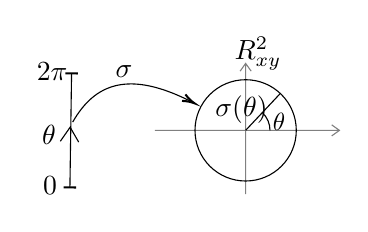
\begin{tikzpicture}[x=0.4pt,y=0.4pt,yscale=-1,xscale=1]
%uncomment if require: \path (0,300); %set diagram left start at 0, and has height of 300

%Shape: Axis 2D [id:dp22600225576346522] 
\draw [color={rgb, 255:red, 128; green, 128; blue, 128 }  ,draw opacity=1 ] (138.75,129.47) -- (305.5,129.47)(220.75,69) -- (220.75,187) (298.5,124.47) -- (305.5,129.47) -- (298.5,134.47) (215.75,76) -- (220.75,69) -- (225.75,76)  ;
%Straight Lines [id:da7351534427888068] 
\draw    (63.5,78) -- (62,181) ;
\draw [shift={(62,181)}, rotate = 270.83] [color={rgb, 255:red, 0; green, 0; blue, 0 }  ][line width=0.75]    (0,5.59) -- (0,-5.59)   ;
\draw [shift={(63.5,78)}, rotate = 270.83] [color={rgb, 255:red, 0; green, 0; blue, 0 }  ][line width=0.75]    (0,5.59) -- (0,-5.59)   ;
\draw   (53.34,139.31) -- (62.21,126.63) -- (69.91,140.06) ;
%Curve Lines [id:da006739188752353686] 
\draw    (64.5,122) .. controls (84.3,87.35) and (114.88,74.26) .. (172.74,104.08) ;
\draw [shift={(174.5,105)}, rotate = 207.72] [color={rgb, 255:red, 0; green, 0; blue, 0 }  ][line width=0.75]    (10.93,-3.29) .. controls (6.95,-1.4) and (3.31,-0.3) .. (0,0) .. controls (3.31,0.3) and (6.95,1.4) .. (10.93,3.29)   ;

%Shape: Circle [id:dp24247899473747292] 
\draw   (175,129.47) .. controls (175,104.2) and (195.48,83.72) .. (220.75,83.72) .. controls (246.02,83.72) and (266.5,104.2) .. (266.5,129.47) .. controls (266.5,154.73) and (246.02,175.22) .. (220.75,175.22) .. controls (195.48,175.22) and (175,154.73) .. (175,129.47) -- cycle ;
%Straight Lines [id:da1420991074145872] 
\draw    (220.75,129.47) -- (251.75,96.47) ;


%Shape: Arc [id:dp4406895489319238] 
\draw  [draw opacity=0] (235.79,113.42) .. controls (240.37,117.7) and (242.74,123.56) .. (242.75,129.47) -- (220.75,129.47) -- cycle ; \draw   (235.79,113.42) .. controls (240.37,117.7) and (242.74,123.56) .. (242.75,129.47) ;

% Text Node
\draw (46,76) node   {$2\pi $};
% Text Node
\draw (44,179) node   {$0$};
% Text Node
\draw (43,134) node   {$\theta $};
% Text Node
\draw (111,76) node   {$\sigma $};
% Text Node
\draw (232,60) node   {$\R^{2}_{xy}$};
% Text Node
\draw (217,111) node   {$\sigma ( \theta )$};
% Text Node
\draw (251,122) node [scale=0.9]  {$\theta $};


\end{tikzpicture}
			\caption{Mapeo de las coordenadas polares.}\label{ch0d6}
		\end{figure}
\end{minipage}}	
 	
 \end{ejem}

%\clase{5}{jueves}{26/9}

\begin{ejem}[caso 2-2]
	Consideremos el rectángulo $\Omega =  [0,2\pi)\t[0,R] $ que es un subconjunto  de $\R^2_{\theta,\rho}$. Sobre este rectángulo tomemos la función $P\colon\Omega\to\R^2_{x,y}$ definida por
	\[ P = \begin{cases}
	x = \rho\cos(\theta) \\
	y = \rho\sin(\theta).
	\end{cases} \]
	Como veremos, esta función $P$ envía el rectángulo $\Omega$ en un disco relleno en $\R^2_{x,y}$ de radio $\rho$ y centrado en el origen.
	
	Para ver esto, consideremos las rectas horizontales $\gamma_\theta$ y las rectas verticales $\gamma_\rho$ definidas por
	\begin{align*}
		\gamma_\theta &= \{(\theta,\rho_0) : 0\leq\theta<2\pi \} \quad\text{( $\rho$ constante)} \\
		\gamma_\rho &= \{(\theta_0,\rho): 0\leq\rho<R \} \quad\text{( $\theta$ constante).}
	\end{align*}
	Veamos ahora la imágen de estas rectas por $P$. La imágen de $\gamma_\theta$ es
%	
\tikzset{every picture/.style={line width=0.75pt}} %set default line width to 0.75pt        
\marginnote{
	\begin{minipage}{5.5cm}
		\begin{figure}[H]\centering
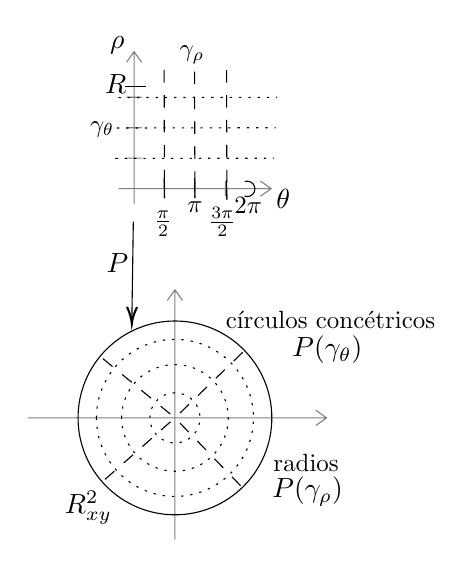
\begin{tikzpicture}[x=0.55pt,y=0.55pt,yscale=-1,xscale=1]
%uncomment if require: \path (0,470); %set diagram left start at 0, and has height of 470

%Shape: Axis 2D [id:dp08602414955349491] 
\draw [color={rgb, 255:red, 128; green, 128; blue, 128 }  ,draw opacity=1 ] (50,178.33) -- (150,178.33)(60,88.33) -- (60,188.33) (143,173.33) -- (150,178.33) -- (143,183.33) (55,95.33) -- (60,88.33) -- (65,95.33) (80,173.33) -- (80,183.33)(100,173.33) -- (100,183.33)(120,173.33) -- (120,183.33)(55,158.33) -- (65,158.33)(55,138.33) -- (65,138.33)(55,118.33) -- (65,118.33) ;
\draw   ;
%Straight Lines [id:da8553900449824685] 
\draw    (67.75,111.5) -- (53.75,111.5) ;


%Shape: Arc [id:dp7042261565620045] 
\draw  [draw opacity=0] (132.73,173.68) .. controls (133.28,173.5) and (133.87,173.41) .. (134.48,173.43) .. controls (137.27,173.52) and (139.47,175.85) .. (139.39,178.65) .. controls (139.3,181.45) and (136.97,183.65) .. (134.17,183.56) .. controls (133.56,183.54) and (132.98,183.42) .. (132.44,183.21) -- (134.32,178.5) -- cycle ; \draw   (132.73,173.68) .. controls (133.28,173.5) and (133.87,173.41) .. (134.48,173.43) .. controls (137.27,173.52) and (139.47,175.85) .. (139.39,178.65) .. controls (139.3,181.45) and (136.97,183.65) .. (134.17,183.56) .. controls (133.56,183.54) and (132.98,183.42) .. (132.44,183.21) ;
%Straight Lines [id:da9840647317250327] 
\draw    (99.96,184.51) -- (99.75,171.5) ;


%Straight Lines [id:da3775217416605612] 
\draw  [dash pattern={on 4.5pt off 4.5pt}]  (99.75,101.5) -- (99.96,184.51) ;


%Straight Lines [id:da9313031352292085] 
\draw    (120.96,185.51) -- (120.75,172.5) ;


%Straight Lines [id:da25043561743865717] 
\draw  [dash pattern={on 4.5pt off 4.5pt}]  (120.75,100.5) -- (120.96,185.51) ;


%Straight Lines [id:da6934472243948512] 
\draw    (79.96,184.51) -- (79.75,171.5) ;


%Straight Lines [id:da44185434524996947] 
\draw  [dash pattern={on 4.5pt off 4.5pt}]  (79.75,100.5) -- (79.96,184.51) ;


%Straight Lines [id:da6388168084335083] 
\draw  [dash pattern={on 0.84pt off 2.51pt}]  (47.75,158.5) -- (152,158.33) ;


%Straight Lines [id:da5836782792660203] 
\draw  [dash pattern={on 0.84pt off 2.51pt}]  (49.75,118.5) -- (154,118.33) ;


%Straight Lines [id:da9986794239727109] 
\draw  [dash pattern={on 0.84pt off 2.51pt}]  (48.75,138.5) -- (153,138.33) ;


%Shape: Axis 2D [id:dp7144990084780382] 
\draw [color={rgb, 255:red, 128; green, 128; blue, 128 }  ,draw opacity=1 ] (-9.55,328.95) -- (186.45,328.95)(86.84,244.83) -- (86.84,409) (179.45,323.95) -- (186.45,328.95) -- (179.45,333.95) (81.84,251.83) -- (86.84,244.83) -- (91.84,251.83)  ;
%Shape: Ellipse [id:dp8667260594865255] 
\draw   (23.18,328.95) .. controls (23.18,293.8) and (51.68,265.3) .. (86.84,265.3) .. controls (121.99,265.3) and (150.49,293.8) .. (150.49,328.95) .. controls (150.49,364.11) and (121.99,392.61) .. (86.84,392.61) .. controls (51.68,392.61) and (23.18,364.11) .. (23.18,328.95) -- cycle ;
%Shape: Ellipse [id:dp9714392583412627] 
\draw  [dash pattern={on 0.84pt off 2.51pt}] (70.34,328.95) .. controls (70.34,319.84) and (77.73,312.46) .. (86.84,312.46) .. controls (95.95,312.46) and (103.34,319.84) .. (103.34,328.95) .. controls (103.34,338.07) and (95.95,345.45) .. (86.84,345.45) .. controls (77.73,345.45) and (70.34,338.07) .. (70.34,328.95) -- cycle ;
%Shape: Circle [id:dp332410896653902] 
\draw  [dash pattern={on 0.84pt off 2.51pt}] (51.79,328.95) .. controls (51.79,309.6) and (67.48,293.91) .. (86.84,293.91) .. controls (106.19,293.91) and (121.88,309.6) .. (121.88,328.95) .. controls (121.88,348.31) and (106.19,364) .. (86.84,364) .. controls (67.48,364) and (51.79,348.31) .. (51.79,328.95) -- cycle ;
%Shape: Ellipse [id:dp9937199373762119] 
\draw  [dash pattern={on 0.84pt off 2.51pt}] (35.25,328.95) .. controls (35.25,300.46) and (58.35,277.37) .. (86.84,277.37) .. controls (115.33,277.37) and (138.42,300.46) .. (138.42,328.95) .. controls (138.42,357.44) and (115.33,380.54) .. (86.84,380.54) .. controls (58.35,380.54) and (35.25,357.44) .. (35.25,328.95) -- cycle ;
%Straight Lines [id:da9578962350159318] 
\draw  [dash pattern={on 4.5pt off 4.5pt}]  (131.36,285.87) -- (86.84,328.95) ;


%Straight Lines [id:da994434191878703] 
\draw  [dash pattern={on 4.5pt off 4.5pt}]  (39.53,290.04) -- (86.84,328.95) ;


%Straight Lines [id:da09208765563112264] 
\draw  [dash pattern={on 4.5pt off 4.5pt}]  (40.92,369.35) -- (86.84,328.95) ;


%Straight Lines [id:da16009223007150286] 
\draw  [dash pattern={on 4.5pt off 4.5pt}]  (129.97,373.52) -- (86.84,328.95) ;


%Straight Lines [id:da032751920105172694] 
\draw    (59.5,200) -- (58.53,265) ;
\draw [shift={(58.5,267)}, rotate = 270.86] [color={rgb, 255:red, 0; green, 0; blue, 0 }  ][line width=0.75]    (10.93,-3.29) .. controls (6.95,-1.4) and (3.31,-0.3) .. (0,0) .. controls (3.31,0.3) and (6.95,1.4) .. (10.93,3.29)   ;


% Text Node
\draw (158,185.33) node   {$\theta $};
% Text Node
\draw (49,84.33) node   {$\rho $};
% Text Node
\draw (48,109.33) node   {$R$};
% Text Node
\draw (135,189.33) node [scale=0.9]  {$2\pi $};
% Text Node
\draw (79,201.33) node [scale=0.9]  {$\frac{\pi }{2}$};
% Text Node
\draw (39,139.33) node [scale=0.9]  {$\gamma _{\theta }$};
% Text Node
\draw (118,200.33) node [scale=0.9]  {$\frac{3\pi }{2}$};
% Text Node
\draw (100,190.33) node [scale=0.9]  {$\pi $};
% Text Node
\draw (98,90.33) node [scale=0.9]  {$\gamma _{\rho }$};
% Text Node
\draw (49,227.33) node   {$P$};
% Text Node
\draw (30,388) node   {$\R^{2}_{xy}$};
% Text Node
\draw (189,264.33) node [scale=0.9] [align=left] {círculos concétricos};
% Text Node
\draw (187,284.33) node   {$P( \gamma _{\theta })$};
% Text Node
\draw (173,358.33) node [scale=0.9] [align=left] {radios};
% Text Node
\draw (174,377.33) node   {$P( \gamma _{\rho })$};


\end{tikzpicture}
	
			\caption{Mapeo de las coordenadas polares (caso 2-2).}\label{ch0d7}
		\end{figure}
\end{minipage}}[-10em]
	\begin{align*}
		P(&\gamma_\theta) = \begin{cases}
		x = \rho_0\cos(\theta) \\
		y = \rho_0\sin(\theta)
		\end{cases} \\
		&\implies \begin{cases}
		x^2 = \rho^2_0\cos^2(\theta) \\
		y^2 = \rho^2_0\sin^2(\theta)
		\end{cases} \\
		&\implies x^2+y^2 = \rho_01,
	\end{align*} 
	que en el plano $\R^2_{x,y}$ describe círculos concéntricos centrados en el orígen de radio $0\leq\rho<R$.
	
	La imágen de $\gamma_\rho$ es
	\begin{align*}
		P(&\gamma_\rho) = \begin{cases}
		x = \rho\cos(\theta_0) \\
		y = \rho\sin(\theta_0)
		\end{cases} \\
		&\implies \frac{y}{x} = \frac{\cancel{\rho}\sin(\theta_0)}{\cancel{\rho}\cos(\theta_0)} \quad \bigg(\rho\neq 0\,\text{y}\, \theta_0\neq \frac{\pi}{2},\frac{3\pi}{2}\bigg) \\
		&\implies \frac{y}{x} = \tan(\theta_0) \\
		&\implies y = \underbrace{\tan(\theta_0)}_m x,
	\end{align*}
	que como se puede ver son rectas con pendiente $\tan(\theta_0)$. Al dar valores a $\theta_0$ se verá que $P(\gamma_\rho) $ describe segmentos de recta en la dirección radial, conformando así ---junto con el resultado de $P(\gamma_\theta)$)--- un disco relleno en $\R^2_{xy}$. El mapeo que describe lo anterior se puede ver en la figura~\ref{ch0d7}. $\mathbb{VIS}$

	
\end{ejem}
\begin{ejem}[cardioides]
	La curva $\rho = b+a\cos(\theta)$ tiene nombres y gráficos diferentes dependiendo de los valores que tomen $a$ y $b$. 
	
	Si $b=a$ entonces $\rho = b\big(1+\cos(\theta)\big)$ describe una \textsc{cardioide}, lo cual se puede ver al darle valores a $\theta$ recordando que este es un ángulo y que $\rho$ es un radio. Su gráfico se puede ver en la figura~\ref{ch0g3}.
	
%			\marginnote{
%		\begin{minipage}{5.5cm}
%			\begin{figure}[H]\centering
%		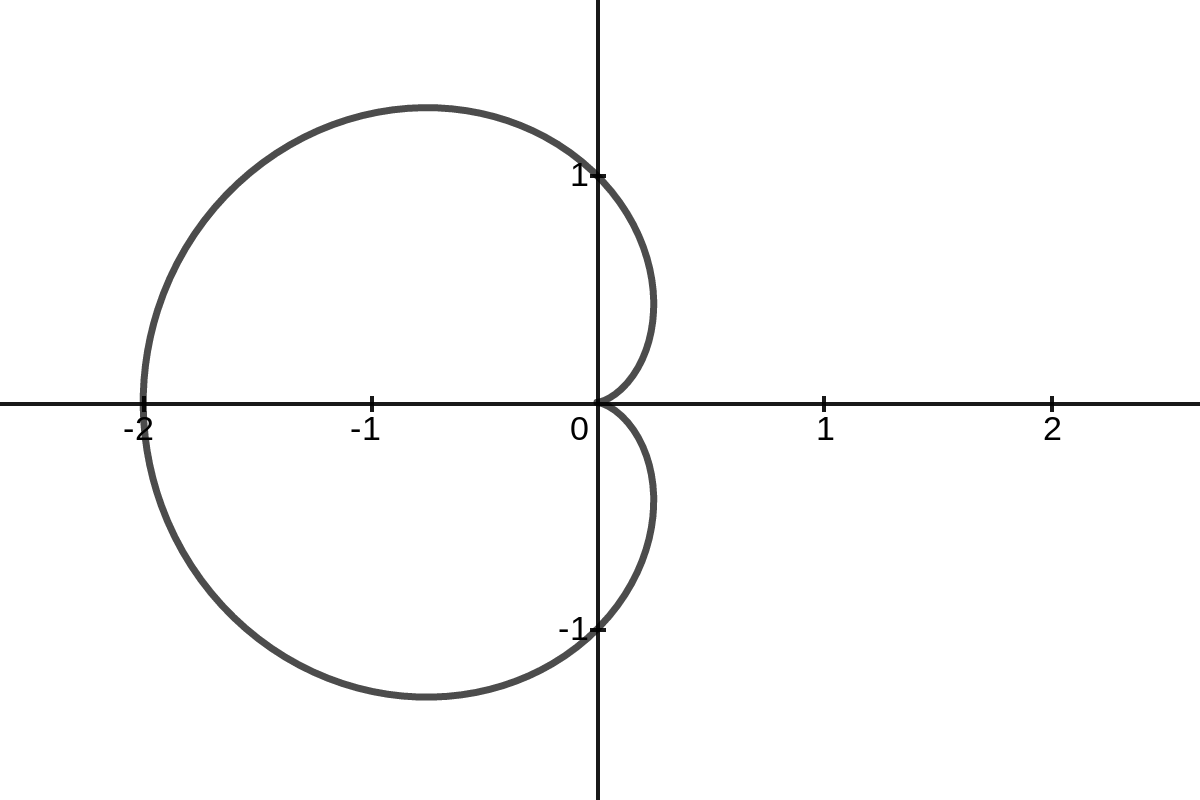
\includegraphics[width=1\linewidth]{pics/c1}\\ 
%\caption{Gráfico de la cardioide con $b=1$}\label{ch0g3}
%			\end{figure}
%	\end{minipage}}
	Si $b>a$ se obtiene una \textsc{cardioide alargada}, que recibe ese nombre debido a que es mas `grande' que la cardiode original y no pasa por el orígen. El hecho de que no pase por el orígen se puede ver rápidamente de la ecuación $0=b+a\cos(\theta)$ que, como los valores extremos del coseno son $-1$ y $1$, no tiene solución para $b>a$. Ver la figura~\ref{ch0g4}.
%			\marginnote{
%		\begin{minipage}{5.5cm}
%			\begin{figure}[H]\centering
%		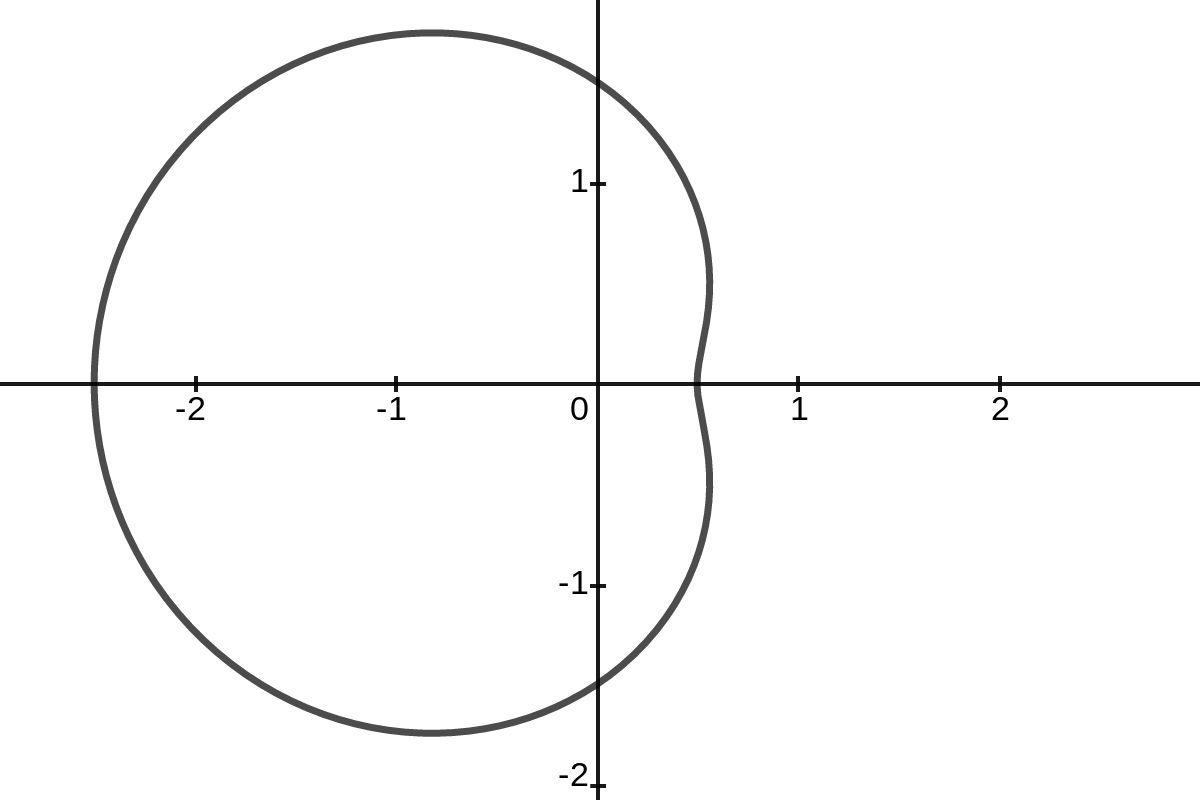
\includegraphics[width=1\linewidth]{pics/c2}\\ 
%\caption{Gráfico de la cardioide alargada con $b=1.5$ y $a=1$}\label{ch0g4}
%			\end{figure}
%	\end{minipage}}[9em]

	Si $b<a$ se obtiene una \textsc{lima\c con}, que se parece a la cardioide pero tiene un bucle cerca del orígen. La causa de este bucle es debido a que, como $b<a$, $\rho$ toma valores negativos cuando $\cos(\theta)<0$.\\
%	\marginnote{
%		\begin{minipage}{5.5cm}
%			\begin{figure}[H]\centering
%				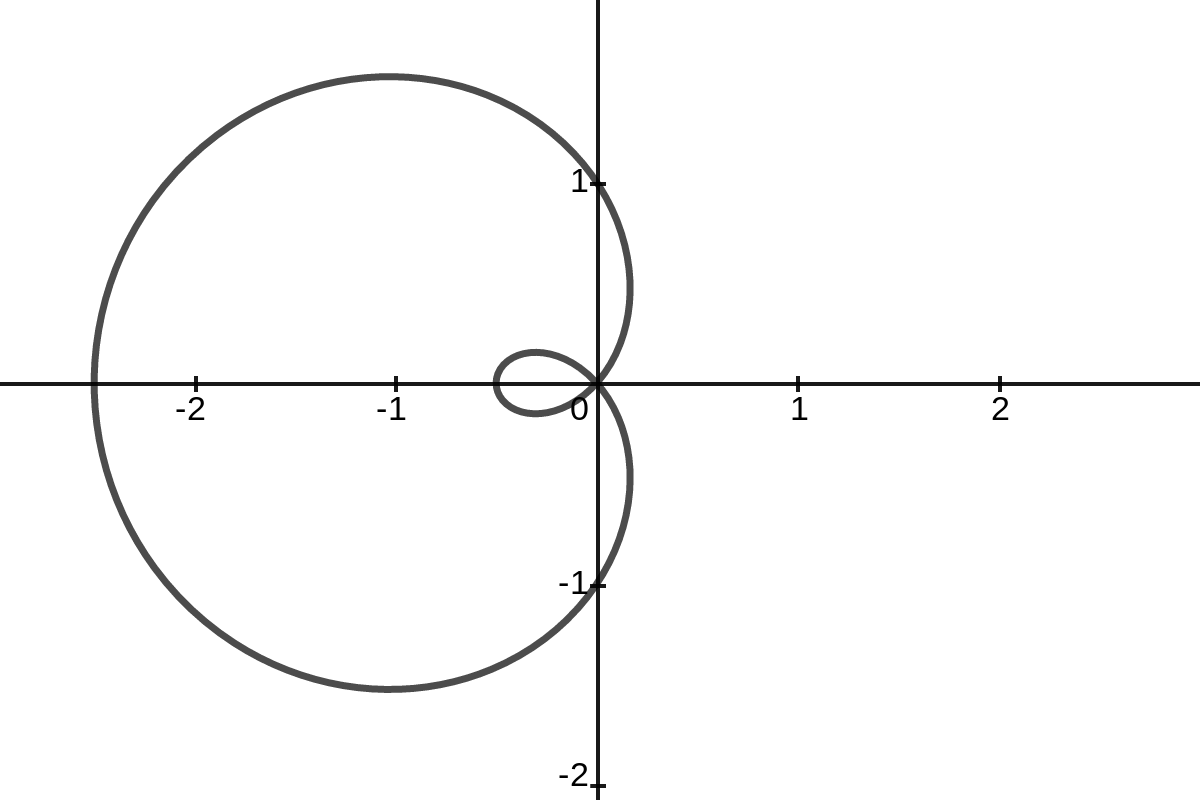
\includegraphics[width=1\linewidth]{pics/c3}\\ 
%				\caption{Gráfico de la lima\c con $b=1$ y $a=1.5$}\label{ch0g5}
%			\end{figure}
%		\end{minipage}}[22em]
\begin{minipage}{.32\linewidth}
	\begin{figure}[H]\centering
		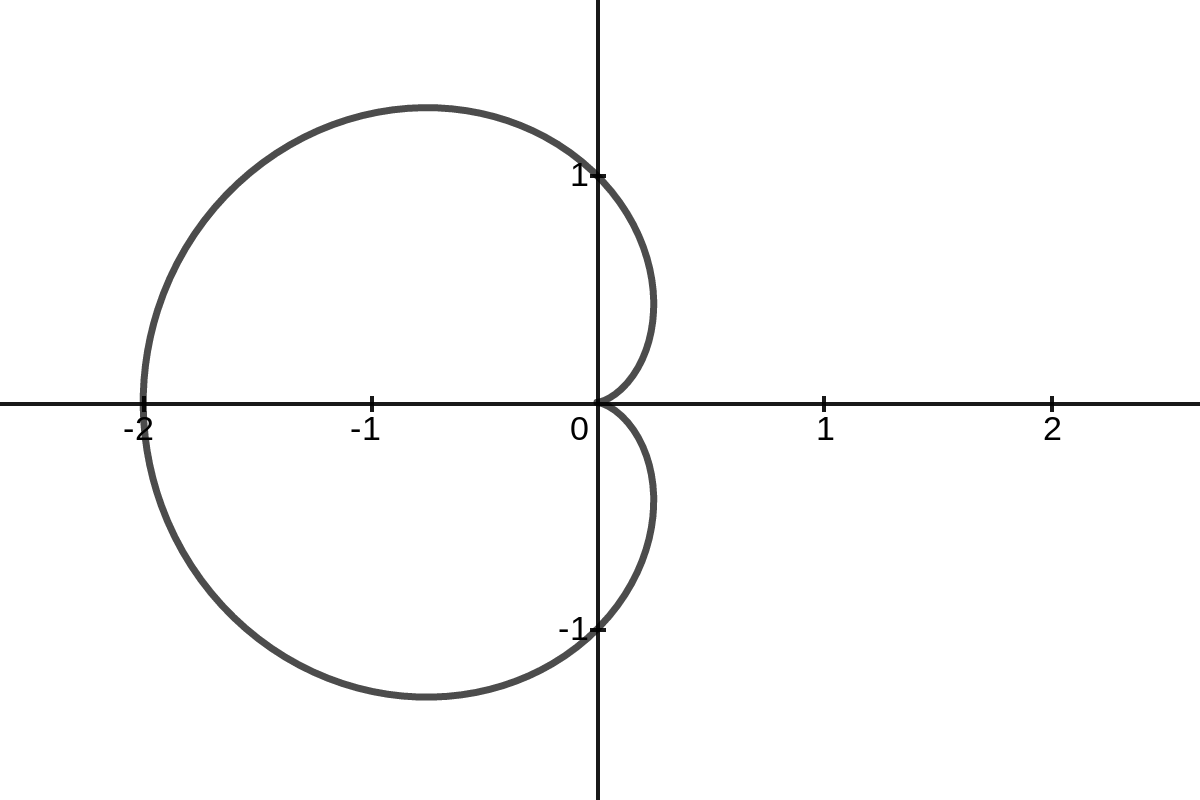
\includegraphics[width=1\linewidth]{pics/c1}\\ 
		\caption{Gráfico de la cardioide con $b=1$}\label{ch0g3}
	\end{figure}
\end{minipage}
\begin{minipage}{.32\linewidth}
	\begin{figure}[H]\centering
		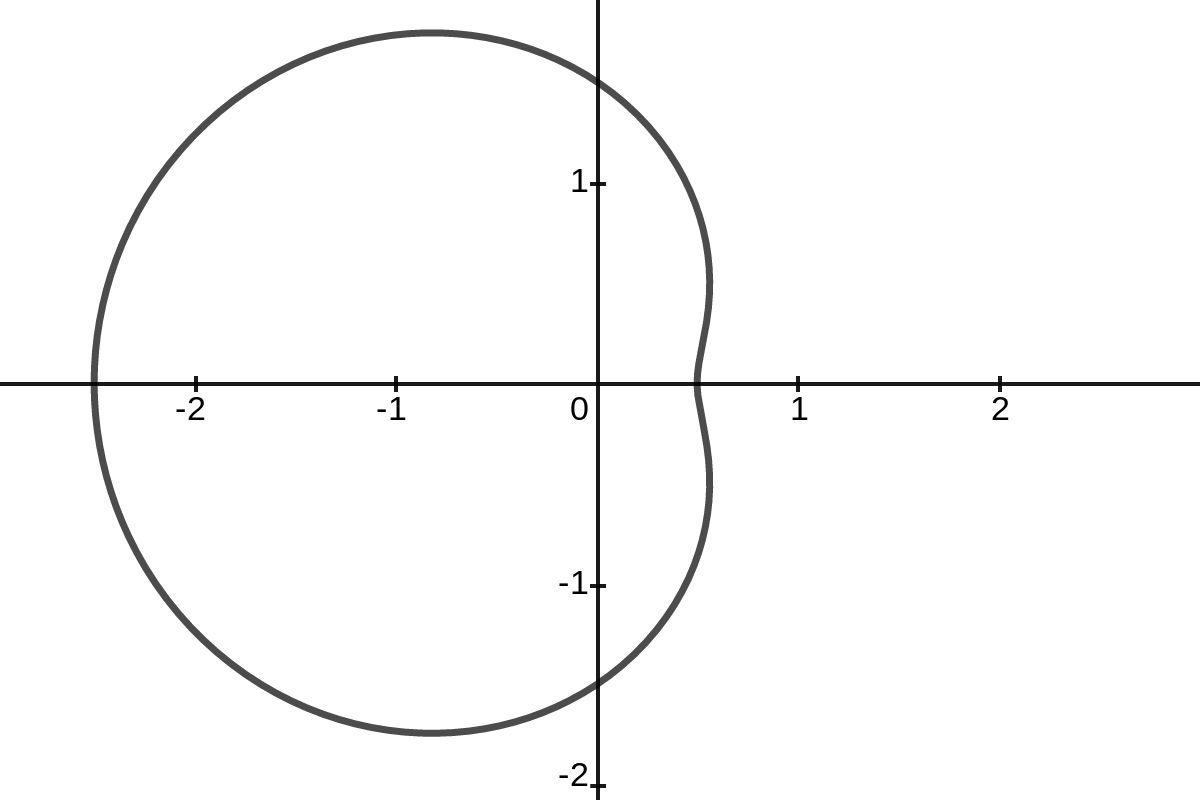
\includegraphics[width=1\linewidth]{pics/c2}\\ 
		\caption{Gráfico de la cardioide alargada con $b=1.5$ y $a=1$}\label{ch0g4}
	\end{figure}
\end{minipage}
\begin{minipage}{.32\linewidth}
	\begin{figure}[H]\centering
		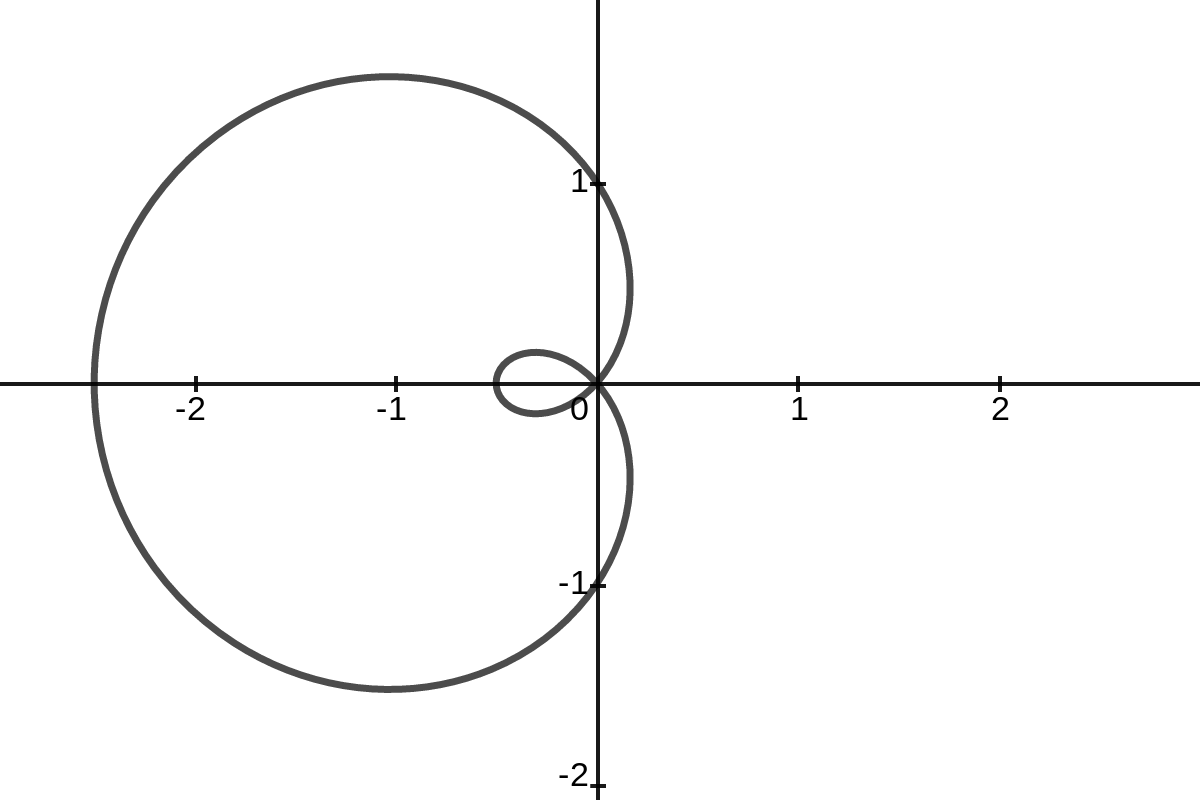
\includegraphics[width=1\linewidth]{pics/c3}\\ 
		\caption{Gráfico de la lima\c con $b=1$ y $a=1.5$}\label{ch0g5}
	\end{figure}
\end{minipage}
\end{ejem}
Para ilustrar la utilidad de las coordenadas polares consideremos su parametrización inversa dada por
\[ P\inv=\begin{cases}
\rho = \sqrt{x^2+y^2} \\[.3em]
\tan(\theta) = \dfrac{y}{x}. 
\end{cases} \]
Es claro que utilizar coordenadas polares para estas curvas es mucho mas fácil de entender y dibujar.

%\clase{6}{viernes}{27/9}

¿Tiene sentido calcular la pendiente $m$ de la recta tangente a $\rho = f(\theta)$ en $\theta=\theta_0$ calculando $m = f'(\theta_0)$?

La respuesta es \emph{no}. Si consideramos la circunferencia $\rho = c$ entonces $f'(\theta_0)=0$, lo cual evidentemente no es cierto. En general $\rho'=f'(\theta_0)$ da el ángulo que forma la recta tangente con el radio vector. 

Lo correcto, en general, es calcular 
\[ m=\frac{\mathrm dy}{\mathrm dx}(x_0,y_0) \]
sabiendo que $x_0=\phi(\theta_0)\cos\theta_0$ y $y_0=\phi(\theta_0)\sin(\theta_0)$. Para calcular esta derivada usamos la regla de la cadena:
\[ \pdd{y}{\theta} = \frac{\mathrm dy}{\mathrm dx}\pdd{x}{\theta}, \]
esto implica que
\begin{align*}
\frac{\mathrm dy}{\mathrm dx} &= \frac{\partial y/\partial\theta}{\partial x/\partial\theta} \\
&= \frac{\phi'(\theta_0)\sin(\theta_0) + \phi(\theta_0)\cos(\theta_0)}{\phi'(\theta_0)\cos(\theta_0) - \phi(\theta_0)\cos(\theta_0).}
\end{align*}

\begin{ejem}[derivar coordenadas polares]
	Considere\-mos la circunferencia $\rho=c$. Queremos calcular su recta tangente con $\theta_0=\pi/4$. Veamos primero, usando la formula anterior,
	\begin{align*}
		\frac{\mathrm dy}{\mathrm dx}\bigg(\frac \pi 4\bigg) &= \frac{\phi'(\pi/4)\sin(\pi/4) + \phi(\pi/4)\cos(\pi/4)}{\phi'(\pi/4)\cos(\pi/4) - \phi(\pi/4)\cos(\pi/4)} \\
		&= \frac{\sqrt 2}{2}  \frac{\phi'(\pi/4) + \phi(\pi/4)}{\phi'(\pi/4) - \phi(\pi/4)} \\
		&= -1.
	\end{align*}
	Ahora, para la ecuación de la recta tenemos que
	\[ y-y_0 = m(x-x_0) \]
	implica
    \begin{align*}
    	&\phantom{\implies}\hspace{.6em} y-y(\theta_0,\rho_0) = \frac{\mathrm dy}{\mathrm dx} \big(x-x(\theta_0,\rho_0)\big) \\
    	&\implies y-y(\pi/4,c) = \frac{\mathrm dy}{\mathrm dx} \big(x-x(\pi/4,c)\big)\\
    	&\implies y -\frac{c}{\sqrt 2} = -1\bigg(x-\frac{c}{\sqrt 2}\bigg) \\
    	&\implies x+y = c\sqrt 2.
    \end{align*}
    Lo anterior se puede ver gráficamente en la figura~\ref{ch0d8}.
%    
\tikzset{every picture/.style={line width=0.75pt}} %set default line width to 0.75pt        
\marginnote{
	\begin{minipage}{5.5cm}
		\begin{figure}[H]\centering
	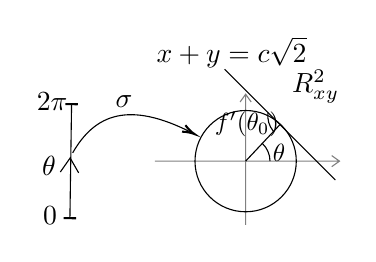
\begin{tikzpicture}[x=0.4pt,y=0.4pt,yscale=-1,xscale=1]
	%uncomment if require: \path (0,300); %set diagram left start at 0, and has height of 300
	
	%Shape: Axis 2D [id:dp8906481887439197] 
	\draw [color={rgb, 255:red, 128; green, 128; blue, 128 }  ,draw opacity=1 ] (138.75,129.47) -- (305.5,129.47)(220.75,69) -- (220.75,187) (298.5,124.47) -- (305.5,129.47) -- (298.5,134.47) (215.75,76) -- (220.75,69) -- (225.75,76)  ;
	%Straight Lines [id:da41323435357946325] 
	\draw    (63.5,78) -- (62,181) ;
	\draw [shift={(62,181)}, rotate = 270.83] [color={rgb, 255:red, 0; green, 0; blue, 0 }  ][line width=0.75]    (0,5.59) -- (0,-5.59)   ;
	\draw [shift={(63.5,78)}, rotate = 270.83] [color={rgb, 255:red, 0; green, 0; blue, 0 }  ][line width=0.75]    (0,5.59) -- (0,-5.59)   ;
	\draw   (53.34,139.31) -- (62.21,126.63) -- (69.91,140.06) ;
	%Curve Lines [id:da5284090654905907] 
	\draw    (64.5,122) .. controls (84.3,87.35) and (114.88,74.26) .. (172.74,104.08) ;
	\draw [shift={(174.5,105)}, rotate = 207.72] [color={rgb, 255:red, 0; green, 0; blue, 0 }  ][line width=0.75]    (10.93,-3.29) .. controls (6.95,-1.4) and (3.31,-0.3) .. (0,0) .. controls (3.31,0.3) and (6.95,1.4) .. (10.93,3.29)   ;
	
	%Shape: Circle [id:dp5870738771744217] 
	\draw   (175,129.47) .. controls (175,104.2) and (195.48,83.72) .. (220.75,83.72) .. controls (246.02,83.72) and (266.5,104.2) .. (266.5,129.47) .. controls (266.5,154.73) and (246.02,175.22) .. (220.75,175.22) .. controls (195.48,175.22) and (175,154.73) .. (175,129.47) -- cycle ;
	%Straight Lines [id:da5762242177877559] 
	\draw    (220.75,129.47) -- (251.75,96.47) ;
	
	
	%Shape: Arc [id:dp37152394327579097] 
	\draw  [draw opacity=0] (235.79,113.42) .. controls (240.37,117.7) and (242.74,123.56) .. (242.75,129.47) -- (220.75,129.47) -- cycle ; \draw   (235.79,113.42) .. controls (240.37,117.7) and (242.74,123.56) .. (242.75,129.47) ;
	%Straight Lines [id:da9773495598747022] 
	\draw    (201.75,46.47) -- (301.75,146.47) ;
	
	
	%Shape: Arc [id:dp9224603848575323] 
	\draw  [draw opacity=0] (245.81,102.5) .. controls (241.81,97.68) and (240.19,91.57) .. (240.93,85.71) -- (262.75,88.47) -- cycle ; \draw   (245.81,102.5) .. controls (241.81,97.68) and (240.19,91.57) .. (240.93,85.71) ;
	
	% Text Node
	\draw (46,76) node   {$2\pi $};
	% Text Node
	\draw (44,179) node   {$0$};
	% Text Node
	\draw (43,134) node   {$\theta $};
	% Text Node
	\draw (111,76) node   {$\sigma $};
	% Text Node
	\draw (284,62) node   {$\R^{2}_{xy}$};
	% Text Node
	\draw (251,122) node [scale=0.9]  {$\theta $};
	% Text Node
	\draw (208,31) node   {$x+y=c\sqrt{2}$};
	% Text Node
	\draw (222,96) node [scale=0.9]  {$f'( \theta _{0})$};
	
	
	\end{tikzpicture}
			\caption{Mapeo de una parametrización.}\label{ch0d8}
		\end{figure}
\end{minipage}}
\end{ejem}
\begin{ejem}[derivar coordenadas polares]
	Hallar en coordenadas polares las rectas tangentes a la lemniscata de Bernoulli
	\[( x^2+y^2)^2 = a(x^2-y^2) \]
	en el origen.
	Sustituyendo los valores de coordenadas polares $x=\cos(\theta)$ y $y=\sin(\theta)$ en la ecuación de la lenmiscata obtenemos
	\begin{align*}
		&\phantom{\implies}\hspace{.6em} \rho^4 = a^2\big(\rho^2\cos^2(\theta) - \rho^2\sin^2(\theta)\big) \\
		&\implies \rho^4 = a^2\rho^2\cos(2\theta)\footnotemark \\
		&\implies \rho^4 - a^2\rho^2\cos(2\theta) = 0 \\
		&\implies \rho^2 \big(\rho^2 - a^2\cos(2\theta)\big) = 0.
	\end{align*}
	\footnotetext{Los $\rho$ no se pueden cancelar porque es un polinomia  de grado 4.}\
	De la última implicación se sigue que
	\[ \rho^2 = 0 \quad\text{o}\quad \rho^2 = a^2\cos(2\theta). \]
	Si $\rho^2 = a^2\cos(2\theta)$ entonces $\rho=\sqrt{\cos(2\theta)}$ y para que esta raiz exista debemos tener $\cos(2\theta)>0$, es decir, $\theta\in[0,\pi/4]\cup[3\pi/4,\pi]$. De donde las rectas tangentes en el origen son $y=\pm x$, como se ve en el gráfico~\ref{ch0g6}.
		\begin{center}
			\begin{minipage}{.5\linewidth}
		\begin{figure}[H]\centering
			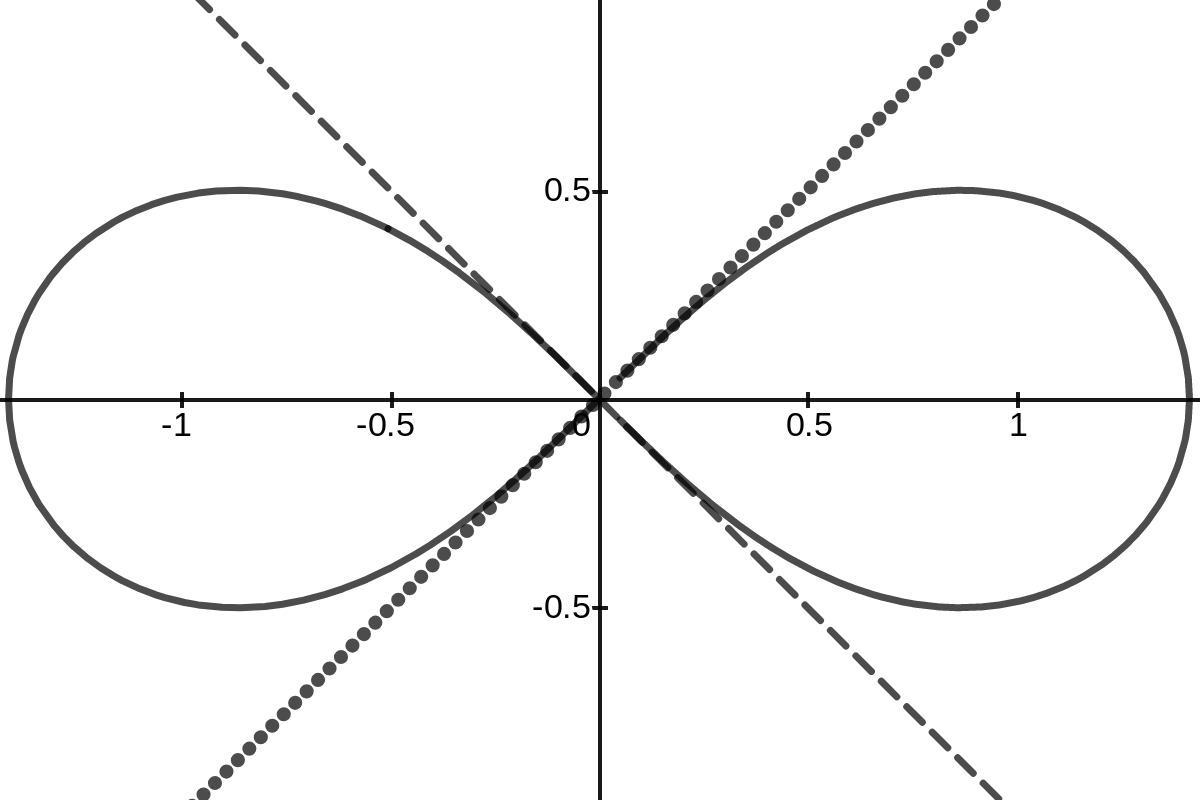
\includegraphics[width=1\linewidth]{pics/l1}\\ 
			\caption{Gráfico de la lemniscata con $a=1$ y sus rectas tangentes en el origen.}\label{ch0g6}
		\end{figure}
	\end{minipage}
		\end{center}
\end{ejem}

\begin{samepage}
	%\clase{7}{martes}{01/10}
	\subsection{Coordenadas Cilíndricas}
\end{samepage}

\noindent
Sea $F(x,y) = 0$ una superficie en $\R^2$ y sea $\sigma\colon\R_t\to\R^2_{xy}$ una parametrización de $F$ dada por $\sigma\big(f(t),g(t)\big)$. Un \textsc{cilindro abstracto} es un punto $(x,y,z)$ tal que $\forall\,z\in\R:(x,y)\in\{F(x,y)=0\}.$ 

Sea $\Phi$ es producto exterior:
\[ \Phi(t,z) = \underbrace{(f(t),g(t),0)}_{\Phi_t}\t\underbrace{(0,0,z)}_{\Phi_z} \]
y esto es si, y solo si,
\begin{align}
	\Phi = \begin{cases}
	x=f(t) \\
	y=g(t) \\
	z=z.
	\end{cases}\label{cilincoord}
\end{align}
La representación gráfica de lo anterior esta en la figura~\ref{ch0d9}.  
%
\tikzset{every picture/.style={line width=0.75pt}} %set default line width to 0.75pt        
\marginnote{
	\begin{minipage}{5.5cm}
		\begin{figure}[H]\centering
	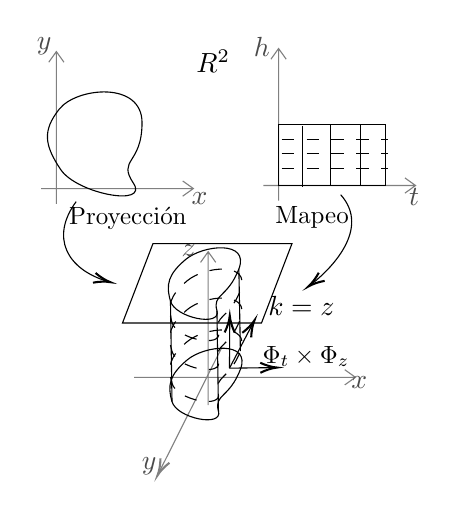
\begin{tikzpicture}[x=0.55pt,y=0.55pt,yscale=-1,xscale=1]
	%uncomment if require: \path (0,300); %set diagram left start at 0, and has height of 300
	
	%Shape: Axis 2D [id:dp0671023438890539] 
	\draw [color={rgb, 255:red, 128; green, 128; blue, 128 }  ,draw opacity=1 ] (23,103.33) -- (123,103.33)(33,13.33) -- (33,113.33) (116,98.33) -- (123,103.33) -- (116,108.33) (28,20.33) -- (33,13.33) -- (38,20.33)  ;
	%Shape: Axis 2D [id:dp4356880068192882] 
	\draw [color={rgb, 255:red, 128; green, 128; blue, 128 }  ,draw opacity=1 ] (169,101.33) -- (269,101.33)(179,11.33) -- (179,111.33) (262,96.33) -- (269,101.33) -- (262,106.33) (174,18.33) -- (179,11.33) -- (184,18.33)  ;
	%Shape: Regular Polygon [id:dp83345563817431] 
	\draw   (34.93,51.11) .. controls (46.22,36.85) and (89.29,32.45) .. (89.29,60.03) .. controls (89.29,87.61) and (72.97,83.82) .. (83.61,99.78) .. controls (94.25,115.74) and (46.45,106.75) .. (35.81,90.79) .. controls (25.18,74.83) and (23.65,65.36) .. (34.93,51.11) -- cycle ;
	%Shape: Rectangle [id:dp9058281148634225] 
	\draw   (179,61.33) -- (249,61.33) -- (249,101.33) -- (179,101.33) -- cycle ;
	%Shape: Boxed Line [id:dp7517627309771912] 
	\draw  [dash pattern={on 4.5pt off 4.5pt}]  (181,90.33) -- (251,90.33) ;
	
	
	%Shape: Boxed Line [id:dp23509819907190233] 
	\draw  [dash pattern={on 4.5pt off 4.5pt}]  (181,80.33) -- (251,80.33) ;
	
	
	%Shape: Boxed Line [id:dp965403871016088] 
	\draw  [dash pattern={on 4.5pt off 4.5pt}]  (181,71.33) -- (251,71.33) ;
	
	
	%Shape: Boxed Bezier Curve [id:dp36220731772572023] 
	\draw    (46.01,111.91) .. controls (28.88,135.18) and (39.6,156.29) .. (66.78,164.36) ;
	\draw [shift={(68.46,164.83)}, rotate = 195.12] [color={rgb, 255:red, 0; green, 0; blue, 0 }  ][line width=0.75]    (10.93,-3.29) .. controls (6.95,-1.4) and (3.31,-0.3) .. (0,0) .. controls (3.31,0.3) and (6.95,1.4) .. (10.93,3.29)   ;
	
	%Curve Lines [id:da22018553388559514] 
	\draw    (219.82,107.38) .. controls (239.91,129.9) and (213.07,156.6) .. (200.04,166.57) ;
	\draw [shift={(198.48,167.72)}, rotate = 324.06] [color={rgb, 255:red, 0; green, 0; blue, 0 }  ][line width=0.75]    (10.93,-3.29) .. controls (6.95,-1.4) and (3.31,-0.3) .. (0,0) .. controls (3.31,0.3) and (6.95,1.4) .. (10.93,3.29)   ;
	
	%Shape: Axis 2D [id:dp9422983370355091] 
	\draw [color={rgb, 255:red, 128; green, 128; blue, 128 }  ,draw opacity=1 ] (84.09,227.33) -- (229.48,227.33)(132.75,144.83) -- (132.75,245.64) (222.48,222.33) -- (229.48,227.33) -- (222.48,232.33) (127.75,151.83) -- (132.75,144.83) -- (137.75,151.83)  ;
	%Shape: Boxed Line [id:dp6413257186656189] 
	\draw  [color={rgb, 255:red, 128; green, 128; blue, 128 }  ,draw opacity=1 ]  (141.56,208) -- (100.34,290.02) ;
	\draw [shift={(99.44,291.8)}, rotate = 296.68] [color={rgb, 255:red, 0; green, 0; blue, 0 }  ] [color={rgb, 255:red, 128; green, 128; blue, 128 }  ,draw opacity=1 ] [line width=0.75]    (10.93,-3.29) .. controls (6.95,-1.4) and (3.31,-0.3) .. (0,0) .. controls (3.31,0.3) and (6.95,1.4) .. (10.93,3.29)   ;
	
	%Shape: Regular Polygon [id:dp8444781340424307] 
	\draw   (117.86,149.99) .. controls (129.39,140.18) and (160.19,137.15) .. (152.91,156.13) .. controls (145.62,175.11) and (135.39,172.51) .. (138.5,183.49) .. controls (141.6,194.47) and (111.09,188.28) .. (107.98,177.3) .. controls (104.88,166.32) and (106.33,159.8) .. (117.86,149.99) -- cycle ;
	%Shape: Rectangle [id:dp08947060083238101] 
	\draw   (96.48,139.48) -- (187.81,139.48) -- (167.77,191.67) -- (76.45,191.67) -- cycle ;
	
	%Shape: Regular Polygon [id:dp765934209815841] 
	\draw   (118.86,215.99) .. controls (130.39,206.18) and (161.19,203.15) .. (153.91,222.13) .. controls (146.62,241.11) and (136.39,238.51) .. (139.5,249.49) .. controls (142.6,260.47) and (112.09,254.28) .. (108.98,243.3) .. controls (105.88,232.32) and (107.33,225.8) .. (118.86,215.99) -- cycle ;
	%Shape: Regular Polygon [id:dp8164080160304793] 
	\draw  [dash pattern={on 4.5pt off 4.5pt}] (118.86,203.99) .. controls (130.39,194.18) and (161.19,191.15) .. (153.91,210.13) .. controls (146.62,229.11) and (136.39,226.51) .. (139.5,237.49) .. controls (142.6,248.47) and (112.09,242.28) .. (108.98,231.3) .. controls (105.88,220.32) and (107.33,213.8) .. (118.86,203.99) -- cycle ;
	%Shape: Regular Polygon [id:dp4699001605273724] 
	\draw  [dash pattern={on 4.5pt off 4.5pt}] (118.86,182.99) .. controls (130.39,173.18) and (161.19,170.15) .. (153.91,189.13) .. controls (146.62,208.11) and (136.39,205.51) .. (139.5,216.49) .. controls (142.6,227.47) and (112.09,221.28) .. (108.98,210.3) .. controls (105.88,199.32) and (107.33,192.8) .. (118.86,182.99) -- cycle ;
	%Shape: Regular Polygon [id:dp7194953751870165] 
	\draw  [dash pattern={on 4.5pt off 4.5pt}] (118.86,163.99) .. controls (130.39,154.18) and (161.19,151.15) .. (153.91,170.13) .. controls (146.62,189.11) and (136.39,186.51) .. (139.5,197.49) .. controls (142.6,208.47) and (112.09,202.28) .. (108.98,191.3) .. controls (105.88,180.32) and (107.33,173.8) .. (118.86,163.99) -- cycle ;
	%Straight Lines [id:da49862726530670776] 
	\draw    (138.5,183.49) -- (139.5,249.49) ;
	
	
	%Straight Lines [id:da113744934569314] 
	\draw    (107.98,177.3) -- (108.98,243.3) ;
	
	
	%Straight Lines [id:da7194247858720582] 
	\draw    (152.91,156.13) -- (153.91,210.13) ;
	
	
	
	%Straight Lines [id:da9241364022526302] 
	\draw    (195,62.33) -- (195,102.33) ;
	
	
	%Straight Lines [id:da342196330864576] 
	\draw    (213,61.33) -- (213,101.33) ;
	
	
	%Straight Lines [id:da4098103221004722] 
	\draw    (233,61.33) -- (233,101.33) ;
	
	
	%Shape: Boxed Line [id:dp18783492901345555] 
	\draw    (146.75,221.33) -- (146.92,188.93) ;
	\draw [shift={(146.93,186.93)}, rotate = 450.31] [color={rgb, 255:red, 0; green, 0; blue, 0 }  ][line width=0.75]    (10.93,-3.29) .. controls (6.95,-1.4) and (3.31,-0.3) .. (0,0) .. controls (3.31,0.3) and (6.95,1.4) .. (10.93,3.29)   ;
	
	%Shape: Boxed Line [id:dp621548564226052] 
	\draw    (146.75,221.33) -- (162.23,191.69) ;
	\draw [shift={(163.15,189.92)}, rotate = 477.57] [color={rgb, 255:red, 0; green, 0; blue, 0 }  ][line width=0.75]    (10.93,-3.29) .. controls (6.95,-1.4) and (3.31,-0.3) .. (0,0) .. controls (3.31,0.3) and (6.95,1.4) .. (10.93,3.29)   ;
	
	%Straight Lines [id:da46586665209900957] 
	\draw    (146.75,221.33) -- (175.93,220.96) ;
	\draw [shift={(177.93,220.93)}, rotate = 539.27] [color={rgb, 255:red, 0; green, 0; blue, 0 }  ][line width=0.75]    (10.93,-3.29) .. controls (6.95,-1.4) and (3.31,-0.3) .. (0,0) .. controls (3.31,0.3) and (6.95,1.4) .. (10.93,3.29)   ;
	
	
	% Text Node
	\draw (127,110) node [color={rgb, 255:red, 74; green, 74; blue, 74 }  ,opacity=1 ]  {$x$};
	% Text Node
	\draw (25,10) node [color={rgb, 255:red, 74; green, 74; blue, 74 }  ,opacity=1 ]  {$y$};
	% Text Node
	\draw (268,109) node [color={rgb, 255:red, 74; green, 74; blue, 74 }  ,opacity=1 ]  {$t$};
	% Text Node
	\draw (168,10) node [color={rgb, 255:red, 74; green, 74; blue, 74 }  ,opacity=1 ]  {$h$};
	% Text Node
	\draw (136,20) node   {$\R^{2}$};
	% Text Node
	\draw (80,123) node [scale=0.9] [align=left] {Proyección};
	% Text Node
	\draw (201,122) node [scale=0.9] [align=left] {Mapeo};
	% Text Node
	\draw (232,231) node [color={rgb, 255:red, 74; green, 74; blue, 74 }  ,opacity=1 ]  {$x$};
	% Text Node
	\draw (94,286) node [color={rgb, 255:red, 74; green, 74; blue, 74 }  ,opacity=1 ]  {$y$};
	% Text Node
	\draw (120,144) node [color={rgb, 255:red, 74; green, 74; blue, 74 }  ,opacity=1 ]  {$z$};
	% Text Node
	\draw (194,180.67) node   {$k=z$};
	% Text Node
	\draw (197,213.65) node [scale=0.9]  {$\Phi _{t} \times \Phi _{z}$};
	
	
	\end{tikzpicture}
			\caption{Mapeo de una parametrización.}\label{ch0d9}
		\end{figure}
\end{minipage}}

\begin{ejem}[cilindro]
	Para el cilindro típico tomemos
	\[ \sigma(t) = \big(R\cos(t),R\sin(t)\big). \]
	Entonces el cilindro queda parametrizado, de acuerdo con~(\ref{cilincoord}), por
	\[ \bm C = \begin{cases}
	x = R\cos(t) \\
	y=R\sin(t) \\
	z=z.
	\end{cases} \]
	
	Su Jacobiano consiste en el producto fundamental:
	\begin{align*}
		\Phi_{t}\t\Phi_{z} &= \begin{vmatrix}
		\ihat& \jhat& \khat \\
		f'(t)& g'(t)& 0 \\
		0& 0& z\\
		\end{vmatrix} \\
		&= \begin{vmatrix}
		g'(t) & 0 \\
		0& 1
		\end{vmatrix}\ihat - \begin{vmatrix}
		f'(t)& 0\\
		0& 1\\
		\end{vmatrix}\jhat - \begin{vmatrix}
		f'(t)& g'(t) \\
		0& 0
		\end{vmatrix}\khat \\
		&=(g'(t),-f'(t),0).
	\end{align*} 
	Y su norma es
	\[ \Norm{\Phi_{t}\t\Phi_{z}} = \sqrt{\big(g'(t)\big)^2+\big(f'(t)\big)^2}. \]
\end{ejem}
\begin{ejem}[Astroide]
	Buscamos el cilindro abstracto cuyas curvas `paralelas' estan determinadas por la \emph{astroide}: $x^{2/3} + y^{2/3} = a^{2/3}$.
	
	Debemos hallar primero una parametrización de esta curva, notemos que
	\begin{align*}
		\phantom{\iff}& a^2 = a^2\cos^2(\theta)+a^2\sin^2(\theta) \\
				  \iff& a^{2/3} = a^{2/3}\big(\cos^6(\theta)\big)^{1/3} + a^{2/3}\big(\sin^6(\theta)\big)^{1/3} \\
				  \iff& a^{2/3} = \underbrace{a^{2/3}\big(\cos^3(\theta)\big)}_x\hspace{0pt}^{2/3} + \underbrace{a^{2/3}\big(\sin^3(\theta)\big)}_y\hspace{0pt}^{2/3} .
	\end{align*}
	Por lo tanto la función $\sigma$ definida por
	\[ \sigma = \begin{cases}
	x = a^{2/3}\cos^3(\theta) \\
	y = a^{2/3}\sin^3(\theta),
	\end{cases} \]
	es una parametrización para la astroide. Luego, por (\ref{cilincoord}), la siguiente $\Phi$
	\[ \Phi = \begin{cases}
	x = a^{2/3}\cos^3(\theta) \quad 0\leq\theta\leq2\pi \\
	y = a^{2/3}\sin^3(\theta) \\
	z=z\phantom{a^{2/3}\sin^3(\theta)} \quad 0\leq z\leq h
	\end{cases} \]
	parametriza el cilindro abstracto que se ve en la figura.
\end{ejem}
\subsection{Coordenadas Cónicas}
\chapter{Integrales de Línea}

\chapter{Integrales de Area}
\noindent	
Como ha ocurrido a lo largo de esta guía, las nociones nuevas de integración en varias variables (en este caso dos variables) recuerdan bastante a las respectivas definiciónes del cálculo en una variable. La definición de integral doble por \emph{sumas de Riemann} sigue esa tendencia y es una extensión natural de las ideas que se encuentran en la definición de intgeral para una variable.

\section{Sumas de Riemann}

\begin{defi}[área]
	Sea $A\subset\R^2$ \emph{acotado}. Supongamos que cada punto $(\bar x_k,\bar y_j)\in A$ tiene la propiedad de pertenecer a un rectángulo de la forma
	\[ \Delta x_k\Delta y_j = [x_{k-1},x_k]\t[y_{j-1},y_j]. \]
	Los puntos extremos del rectángulo anterior $\{(x_k,y_j)| 1\leq k\leq n, 1\leq j\leq m \}$ son una 
	\textup{\textsf{\textsc{partición}}}
	de $A$.
	
	Le asociamos a cada rectángulo antes mencionado un número real no negativo
	\[ \Delta A_{kj} = (x_k-x_{k-1})(y_j-y_{j-1}), \]
	llamado el 
	\textup{\textsf{\textsc{diferencial de área}}}
	del rectángulo. Entonces podemos extender la noción de área de $\R$ a $\R^2$
	\[ \textrm{area} A = \lim\limits_{\substack{m\to\infty \\ n\to\infty}} \sum_{k=1}^{n}\sum_{j=1}^{m}\Delta A_{kj}.  \]
	
	Si los límites anteriores existen y son iguales los denotaremos por el \textsc{área} de $A$:
	\[ \textrm{area} A = \iint_A dA = \iint_A dxdy. \]
\end{defi}
\begin{defi}[integral doble]
	Sean $A\subset\R^2$ y $(\bar x_k,\bar y_j)\in A$ como en la definición anterior. Si $f:A\to\R$ es una función \textsc{continua} entonces definimos la integral doble de $f$ sobre $A$ como
	\begin{align}\label{defiint}
		\iint_A f(x,y)\,dA = \lim_{\substack{n\to\infty \\ m\to\infty}} \sum_{\substack{1\leq k\leq n \\ 1\leq j\leq m}} f(\bar x_k,\bar y_j)\Delta A_{kj}.
	\end{align}
\end{defi}
\begin{ejem}[integral por definición]
	Calcular por definición 
	\[ \iint_{A} xy\,dA \]
	con $A = [0,1]^2$.
	
	Empezamos constuyendo la \emph{partición equi-espaciada} del conjunto $A$ de la siguiente forma:
%\begin{small}
		\begin{multline*}
			x_0=0<x_1=\frac{1}{n}<x_2=\frac{2}{n}\\
			\hspace{6em}<\cdots<x_k=\frac{k}{n}<\cdots\\
			<x_n=\frac{n}{n} =1,
		\end{multline*}
%\end{small}
	análogamente,
%\begin{small}
	\begin{multline*}
		y_0=0<y_1=\frac{1}{m}<y_2=\frac{2}{m}\\
		\hspace{6em}<\cdots<y_k=\frac{k}{m}<\cdots\\
		<y_n=\frac{m}{m} =1.
	\end{multline*}	
%\end{small}
	
	Tomamos ahora como \emph{puntos de muestra} $(\bar x_k,\bar y_j)$ a las esquinas superiores derechas de los rectángulos, es decir, a los puntos $(x_k,y_j)$.
	
	Podemos entonces, teniendo en cuenta que $f(x,y) = xy$ es continua en $A$, usar la ecuación~\ref{defiint}:
	{\allowdisplaybreaks
	\begin{align*}
		\iint_A xy\, dA &= \lim_{\substack{n\to\infty \\ m\to\infty}} \sum_{\substack{1\leq k\leq n \\ 1\leq j\leq m}} f(\bar x_k,\bar y_j)\Delta x_k\Delta y_j \\ 
		&=\lim_{\substack{n\to\infty \\ m\to\infty}} \sum_{\substack{1\leq k\leq n \\ 1\leq j\leq m}} \bar x_k\bar y_j \Delta x_k\Delta y_j \\
		&=\lim_{\substack{n\to\infty \\ m\to\infty}} \sum_{\substack{1\leq k\leq n \\ 1\leq j\leq m}} \frac{k}{n}\frac{j}{m}\frac{1}{n}\frac{1}{m} \\
		&=\lim_{\substack{n\to\infty \\ m\to\infty}} \left(\frac{1}{n^2}\sum_{1\leq k\leq n} k\right)\left(\frac{1}{n^2}\sum_{1\leq j\leq m} j\right) \\
		&=\biggl( \lim\limits_{n\to\infty}\frac{1}{n^2} \big(\frac{n^2}{2}+\frac{n}{2}\big) \biggr)\\
		&\phantom{a}\hspace{6em} \biggl( \lim\limits_{m\to\infty}\frac{1}{m^2} \big(\frac{m^2}{2}+\frac{m}{2}\big) \biggr) \\
		&= \left( \frac{1}{2}+0 \right)\left( \frac{1}{2}+0 \right) \\
		&= \frac{1}{4}.
	\end{align*}}
\end{ejem}

\section{Ejercicios}

\newcommand{\xk}{x_{k}}\newcommand{\xkk}{x_{k-1}}
\newcommand{\yj}{y_{j}}\newcommand{\yjj}{y_{j-1}}
\begin{ejer}
	Sean $A = [a,b]\t[c,d]$ y $a,c$ mayores que cero. Calular por definición 
	\[ \iint_{A} \frac{dA}{x^2\sqrt{y}}, \]
	usando como puntos de muestra
	\[ \bar x_k = \sqrt{\xkk\xk}\quad\text{y}\quad\bar y_j=\left( \frac{\sqrt{\yjj}}{2} - \frac{\sqrt{\yj}}{2} \right)^2. \] 
\end{ejer}
\begin{sol}
	Tomemos la partición de $A$ dada por
	\[ a=x_0<x_1<\cdots<x_n=b \]
	y
	\[ c=y_0<y_1<\cdots<y_m=d. \]
	
	Veamos primero que los puntos sugeridos son en efecto puntos de muestra válidos. Por un lado
	\begin{align*}
		 \xkk&<\xk \\
		\implies \xkk^2 &< \xk\xkk \\
		\implies \xkk &< \sqrt{\xk\xkk},
	\end{align*}
	y también,
	\begin{align*}
		 \xkk&<\xk \\
		\implies\,\phantom{a}\xkk\xk &< \xk^2 \\
		\implies \sqrt{\xkk\xk} &< \xk.
	\end{align*}
	Entonces se tiene que
	\[ \xkk < \sqrt{\xkk\xk} < \xk. \]
	
	Por otro lado
	{\allowdisplaybreaks
	\begin{align*}
	\yjj &< \yj\\
	\implies \frac{\sqrt{\yjj}}{2} &< \frac{\sqrt{\yj}}{2} \\
	\implies \sqrt{\yj} &<  \frac{\sqrt{\yj}}{2} + \frac{\sqrt{\yjj}}{2} \\
	\implies \yjj &< \left( \frac{\sqrt{\yjj}}{2} + \frac{\sqrt{\yj}}{2} \right)^2,
	\end{align*}}
	y también,
	\begin{align*}
		\yjj &< \yj\\
		\implies\hspace{4.3em} \frac{\sqrt{\yjj}}{2} &< \frac{\sqrt{\yj}}{2} \\
		\implies\hspace{1.4em} \frac{\sqrt{\yjj}}{2} + \frac{\sqrt{\yj}}{2} &< \sqrt{\yj} \\
		\implies \left( \frac{\sqrt{\yjj}}{2} + \frac{\sqrt{\yj}}{2} \right)^2 &< \yj.
	\end{align*}
	Por lo tanto
	\[ \yjj < \frac{\sqrt{\yjj}}{2} + \frac{\sqrt{\yj}}{2} < \yj \]
	Entonces los puntos $\bar x_k$ y $\bar y_j$ son en efecto puntos de muestra válidos.
	
	Por lo tanto podemos calcular la integral doble usando la definición, pues la función $f(x,y) = (1/x^2) (1/\sqrt{y})$ es continua debido a que $x,y$ son mayores que cero (y esto es debido a que $a,c$ lo son).
	
	Veamos primero que,
	\begin{align*}
		f(\bar x_k,\bar y_j) &= \left( \sqrt{\xkk\xk}^2 \sqrt{\left( \frac{\sqrt{\yjj}}{2} + \frac{\sqrt{\yj}}{2} \right)^2} \right)\inv  \\
		&= \left( (\xkk\xk) \left( \frac{\sqrt{\yj}}{2} + \frac{\sqrt{\yjj}}{2} \right) \right)\inv \\
		&= \frac{2}{(\xkk\xk) ( \sqrt{\yj} + \sqrt{\yjj})} \\
		&= \frac{2(\sqrt{\yj} - \sqrt{\yjj})}{(\xkk\xk)(\sqrt{\yj} - \sqrt{\yjj}) ( \sqrt{\yj} + \sqrt{\yjj} )} \\
		&= \frac{2(\sqrt{\yj} - \sqrt{\yjj})}{(\xkk\xk)(\yj-\yjj)}.
	\end{align*}
	
	Ahora consideremos la suma:
	{\allowdisplaybreaks
	\begin{align*}
		\sigma&= \sum_{\substack{1\leq k\leq n \\ 1\leq j\leq m}} f(\bar x_k,\bar y_j) (\xk-\xkk)(\yj-\yjj) \\
		&= \sum_{\substack{1\leq k\leq n \\ 1\leq j\leq m}} \frac{2(\sqrt{\yj} - \sqrt{\yjj})}{(\xkk\xk)\cancel{(\yj-\yjj)}} (\xk-\xkk)\cancel{(\yj-\yjj)} \\
		&= \sum_{\substack{1\leq k\leq n \\ 1\leq j\leq m}} \frac{2(\sqrt{\yj} - \sqrt{\yjj})(\xk-\xkk)}{(\xkk\xk)} \\
		&= \sum_{1\leq k\leq n} \frac{\xk-\xkk}{\xk\xkk} \sum_{1\leq j\leq m}2\sqrt{\yj} - 2\sqrt{\yjj} \\
		&= \left( \sum_{1\leq k\leq n} \frac{\cancel{\xk}}{\cancel{\xk}\xkk} - \frac{\cancel{\xkk}}{\xk\cancel{\xkk}} \right) (2\sqrt{y_m}-2\sqrt{y_0}) \\
		&= 2(\sqrt{y_m}-\sqrt{y_0}) \left( \sum_{1\leq k\leq n} \frac{1}{\xkk} - \frac{1}{\xk} \right) \\ 
		&= 2(\sqrt{y_m}-\sqrt{y_0}) \left( \frac{1}{x_0} - \frac{1}{x_n}  \right) \\
		&= 2(\sqrt{d} - \sqrt{c})\left( \frac{1}{a} - \frac{1}{b} \right).
	\end{align*}}

	Luego la integral doble
	\[ \iint_{A} \frac{dA}{x^2\sqrt{y}} = 2(\sqrt{d} - \sqrt{c})\left( \frac{1}{a} - \frac{1}{b} \right) \]
	siempre que $A = [a,b]\t[c,d]$ y $a,c>0$.
\end{sol}

\section{Integrales iteradas}
\section{Integrales por cambio de variable}
\chapter{Integrales de Volumen}
\backmatter
\end{document}